%  LaTeX support: latex@mdpi.com 
%  For support, please attach all files needed for compiling as well as the log file, and specify your operating system, LaTeX version, and LaTeX editor.

%=================================================================
\documentclass[journal,article,submit,pdftex,moreauthors]{Definitions/mdpi} 
\usepackage{amsmath}
\usepackage{algorithm}
\usepackage{algpseudocode}
\usepackage{amssymb}
\usepackage{comment}
\usepackage{amsmath}
\usepackage{tikz}
\usetikzlibrary{shapes.geometric, arrows.meta, positioning, calc, fit}
%\documentclass[preprints,article,submit,pdftex,moreauthors]{Definitions/mdpi} 
% For posting an early version of this manuscript as a preprint, you may use "preprints" as the journal. Changing "submit" to "accept" before posting will remove line numbers.

%--------------------
% Class Options:
%--------------------
%----------
% journal
%----------
% Choose between the following MDPI journals:
% accountaudit, acoustics, actuators, addictions, adhesives, admsci, adolescents, aerobiology, aerospace, agriculture, agriengineering, agrochemicals, agronomy, ai, air, algorithms, allergies, alloys, amh, analytica, analytics, anatomia, anesthres, animals, antibiotics, antibodies, antioxidants, applbiosci, appliedchem, appliedmath, appliedphys, applmech, applmicrobiol, applnano, applsci, aquacj, architecture, arm, arthropoda, arts, asc, asi, astronomy, atmosphere, atoms, audiolres, automation, axioms, bacteria, batteries, bdcc, behavsci, beverages, biochem, bioengineering, biologics, biology, biomass, biomechanics, biomed, biomedicines, biomedinformatics, biomimetics, biomolecules, biophysica, biosensors, biosphere, biotech, birds, blockchains, bloods, blsf, brainsci, breath, buildings, businesses, cancers, carbon, cardiogenetics, catalysts, cells, ceramics, challenges, chemengineering, chemistry, chemosensors, chemproc, children, chips, cimb, civileng, cleantechnol, climate, clinbioenerg, clinpract, clockssleep, cmd, cmtr, coasts, coatings, colloids, colorants, commodities, complications, compounds, computation, computers, condensedmatter, conservation, constrmater, cosmetics, covid, crops, cryo, cryptography, crystals, csmf, ctn, curroncol, cyber, dairy, data, ddc, dentistry, dermato, dermatopathology, designs, devices, diabetology, diagnostics, dietetics, digital, disabilities, diseases, diversity, dna, drones, dynamics, earth, ebj, ecm, ecologies, econometrics, economies, education, eesp, ejihpe, electricity, electrochem, electronicmat, electronics, encyclopedia, endocrines, energies, eng, engproc, ent, entomology, entropy, environments, epidemiologia, epigenomes, esa, est, famsci, fermentation, fibers, fintech, fire, fishes, fluids, foods, forecasting, forensicsci, forests, fossstud, foundations, fractalfract, fuels, future, futureinternet, futureparasites, futurepharmacol, futurephys, futuretransp, galaxies, games, gases, gastroent, gastrointestdisord, gastronomy, gels, genealogy, genes, geographies, geohazards, geomatics, geometry, geosciences, geotechnics, geriatrics, glacies, grasses, greenhealth, gucdd, hardware, hazardousmatters, healthcare, hearts, hemato, hematolrep, heritage, higheredu, highthroughput, histories, horticulturae, hospitals, humanities, humans, hydrobiology, hydrogen, hydrology, hygiene, idr, iic, ijerph, ijfs, ijgi, ijmd, ijms, ijns, ijpb, ijt, ijtm, ijtpp, ime, immuno, informatics, information, infrastructures, inorganics, insects, instruments, inventions, iot, j, jal, jcdd, jcm, jcp, jcs, jcto, jdad, jdb, jeta, jfb, jfmk, jimaging, jintelligence, jlpea, jmahp, jmmp, jmms, jmp, jmse, jne, jnt, jof, joitmc, joma, jop, jor, journalmedia, jox, jpbi, jpm, jrfm, jsan, jtaer, jvd, jzbg, kidney, kidneydial, kinasesphosphatases, knowledge, labmed, laboratories, land, languages, laws, life, lights, limnolrev, lipidology, liquids, literature, livers, logics, logistics, lubricants, lymphatics, machines, macromol, magnetism, magnetochemistry, make, marinedrugs, materials, materproc, mathematics, mca, measurements, medicina, medicines, medsci, membranes, merits, metabolites, metals, meteorology, methane, metrics, metrology, micro, microarrays, microbiolres, microelectronics, micromachines, microorganisms, microplastics, microwave, minerals, mining, mmphys, modelling, molbank, molecules, mps, msf, mti, multimedia, muscles, nanoenergyadv, nanomanufacturing, nanomaterials, ncrna, ndt, network, neuroglia, neurolint, neurosci, nitrogen, notspecified, nursrep, nutraceuticals, nutrients, obesities, oceans, ohbm, onco, oncopathology, optics, oral, organics, organoids, osteology, oxygen, parasites, parasitologia, particles, pathogens, pathophysiology, pediatrrep, pets, pharmaceuticals, pharmaceutics, pharmacoepidemiology, pharmacy, philosophies, photochem, photonics, phycology, physchem, physics, physiologia, plants, plasma, platforms, pollutants, polymers, polysaccharides, populations, poultry, powders, preprints, proceedings, processes, prosthesis, proteomes, psf, psych, psychiatryint, psychoactives, psycholint, publications, purification, quantumrep, quaternary, qubs, radiation, reactions, realestate, receptors, recycling, regeneration, religions, remotesensing, reports, reprodmed, resources, rheumato, risks, robotics, rsee, ruminants, safety, sci, scipharm, sclerosis, seeds, sensors, separations, sexes, signals, sinusitis, siuj, skins, smartcities, sna, societies, socsci, software, soilsystems, solar, solids, spectroscj, sports, standards, stats, std, stresses, surfaces, surgeries, suschem, sustainability, symmetry, synbio, systems, tae, targets, taxonomy, technologies, telecom, test, textiles, thalassrep, therapeutics, thermo, timespace, tomography, tourismhosp, toxics, toxins, transplantology, transportation, traumacare, traumas, tropicalmed, universe, urbansci, uro, vaccines, vehicles, venereology, vetsci, vibration, virtualworlds, viruses, vision, waste, water, wem, wevj, wild, wind, women, world, youth, zoonoticdis

%---------
% article
%---------
% The default type of manuscript is "article", but can be replaced by: 
% abstract, addendum, article, benchmark, book, bookreview, briefcommunication, briefreport, casereport, changes, clinicopathologicalchallenge, comment, commentary, communication, conceptpaper, conferenceproceedings, correction, conferencereport, creative, datadescriptor, discussion, entry, expressionofconcern, extendedabstract, editorial, essay, erratum, fieldguide, hypothesis, interestingimages, letter, meetingreport, monograph, newbookreceived, obituary, opinion, proceedingpaper, projectreport, reply, retraction, review, perspective, protocol, shortnote, studyprotocol, supfile, systematicreview, technicalnote, viewpoint, guidelines, registeredreport, tutorial,  giantsinurology, urologyaroundtheworld
% supfile = supplementary materials

%----------
% submit
%----------
% The class option "submit" will be changed to "accept" by the Editorial Office when the paper is accepted. This will only make changes to the frontpage (e.g., the logo of the journal will get visible), the headings, and the copyright information. Also, line numbering will be removed. Journal info and pagination for accepted papers will also be assigned by the Editorial Office.

%------------------
% moreauthors
%------------------
% If there is only one author the class option oneauthor should be used. Otherwise use the class option moreauthors.

%---------
% pdftex
%---------
% The option pdftex is for use with pdfLaTeX. Remove "pdftex" for (1) compiling with LaTeX & dvi2pdf (if eps figures are used) or for (2) compiling with XeLaTeX.

%=================================================================
% MDPI internal commands - do not modify
\firstpage{1} 
\makeatletter 
\setcounter{page}{\@firstpage} 
\makeatother
\pubvolume{1}
\issuenum{1}
\articlenumber{0}
\pubyear{2025}
\copyrightyear{2025}
%\externaleditor{Firstname Lastname} % More than 1 editor, please add `` and '' before the last editor name
\datereceived{ } 
\daterevised{ } % Comment out if no revised date
\dateaccepted{ } 
\datepublished{ } 
%\datecorrected{} % For corrected papers: "Corrected: XXX" date in the original paper.
%\dateretracted{} % For retracted papers: "Retracted: XXX" date in the original paper.
\hreflink{https://doi.org/} % If needed use \linebreak
%\doinum{}
%\pdfoutput=1 % Uncommented for upload to arXiv.org
%\CorrStatement{yes}  % For updates
%\longauthorlist{yes} % For many authors that exceed the left citation part
%\IsAssociation{yes} % For association journals

%=================================================================
% Add packages and commands here. The following packages are loaded in our class file: fontenc, inputenc, calc, indentfirst, fancyhdr, graphicx, epstopdf, lastpage, ifthen, float, amsmath, amssymb, lineno, setspace, enumitem, mathpazo, booktabs, titlesec, etoolbox, tabto, xcolor, colortbl, soul, multirow, microtype, tikz, totcount, changepage, attrib, upgreek, array, tabularx, pbox, ragged2e, tocloft, marginnote, marginfix, enotez, amsthm, natbib, hyperref, cleveref, scrextend, url, geometry, newfloat, caption, draftwatermark, seqsplit
% cleveref: load \crefname definitions after \begin{document}

%=================================================================
% Please use the following mathematics environments: Theorem, Lemma, Corollary, Proposition, Characterization, Property, Problem, Example, ExamplesandDefinitions, Hypothesis, Remark, Definition, Notation, Assumption
%% For proofs, please use the proof environment (the amsthm package is loaded by the MDPI class).

%=================================================================
% Full title of the paper (Capitalized)
\Title{Joint UAV Trajectory Planning and LEO Satellite  Selection for Data Offloading in Space-Air-Ground  Integrated Networks}

% MDPI internal command: Title for citation in the left column
\TitleCitation{Joint UAV Trajectory Planning and LEO Satellite  Selection for Data Offloading in Space-Air-Ground  Integrated Networks}

% Author Orchid ID: enter ID or remove command
\newcommand{\orcidauthorA}{0000-0003-3080-1514} % Add \orcidA{} behind the author's name
%\newcommand{\orcidauthorB}{0000-0000-0000-000X} % Add \orcidB{} behind the author's name

% Authors, for the paper (add full first names)
\Author{Tie Liu $^{1}$\orcidA{}, Firstname Lastname $^{2}$ and Firstname Lastname $^{2,}$*}

%\longauthorlist{yes}

% MDPI internal command: Authors, for metadata in PDF
\AuthorNames{Tie Liu, Firstname Lastname and Firstname Lastname}

% Author citation:  
\AuthorCitation{L, Tie.; Lastname, F.; Lastname, F.}

% Affiliations / Addresses (Add [1] after \address if there is only one affiliation.)
\address{%
$^{1}$ \quad Affiliation 1; e-mail@e-mail.com\\
$^{2}$ \quad Affiliation 2; e-mail@e-mail.com}

% Contact information of the corresponding author
\corres{Correspondence: e-mail@e-mail.com; Tel.: (optional; include country code; if there are multiple corresponding authors, add author initials) +xx-xxxx-xxx-xxxx (F.L.)}

% Current address and/or shared authorship
%\firstnote{Current address: Affiliation.}  
% Current address should not be the same as any items in the Affiliation section.

%\secondnote{These authors contributed equally to this work.}
% The commands \thirdnote{} till \eighthnote{} are available for further notes.

%\simplesumm{} % Simple summary

%\conference{} % An extended version of a conference paper

% Abstract (Do not insert blank lines, i.e. \\) 
\abstract{With the development of low earth orbit (LEO) satellites and unmanned aerial vehicles (UAVs), the space-airground integrated network (SAGIN) becomes a major trend in the next-generation networks.However, due to the instability of heterogeneous communication and time-varying characteristics of SAGIN, it is challenging to meet the remote Internet of Things (IoT) demands for data collection and offloading.In this paper, we investigate a two-phase hierarchical data uplink model in SAGIN. Specifically, UAVs optimize trajectories to enable efficient data collection from IoT devices, and then they transmit the data to LEO satellites with computing capabilities for further processing.The problem is formulated to minimize the total energy consumption for UAVs and the packet loss rate transmitted to LEO satellites.Ultimately, simulation results demonstrate the effectiveness of the proposed algorithm, which reduces energy consumption by approximately 10\% compared to the baseline algorithm and lowers the packet loss rate by an average of 3 to 5 times.}

% Keywords
\keyword{SAGIN, UAV, LEO satellite, data offloading.} 

% The fields PACS, MSC, and JEL may be left empty or commented out if not applicable
%\PACS{J0101}
%\MSC{}
%\JEL{}

%%%%%%%%%%%%%%%%%%%%%%%%%%%%%%%%%%%%%%%%%%
% Only for the journal Diversity
%\LSID{\url{http://}}

%%%%%%%%%%%%%%%%%%%%%%%%%%%%%%%%%%%%%%%%%%
% Only for the journal Applied Sciences
%\featuredapplication{Authors are encouraged to provide a concise description of the specific application or a potential application of the work. This section is not mandatory.}
%%%%%%%%%%%%%%%%%%%%%%%%%%%%%%%%%%%%%%%%%%

%%%%%%%%%%%%%%%%%%%%%%%%%%%%%%%%%%%%%%%%%%
% Only for the journal Data
%\dataset{DOI number or link to the deposited data set if the data set is published separately. If the data set shall be published as a supplement to this paper, this field will be filled by the journal editors. In this case, please submit the data set as a supplement.}
%\datasetlicense{License under which the data set is made available (CC0, CC-BY, CC-BY-SA, CC-BY-NC, etc.)}

%%%%%%%%%%%%%%%%%%%%%%%%%%%%%%%%%%%%%%%%%%
% Only for the journal BioTech, Fishes, Neuroimaging and Toxins
%\keycontribution{The breakthroughs or highlights of the manuscript. Authors can write one or two sentences to describe the most important part of the paper.}

%%%%%%%%%%%%%%%%%%%%%%%%%%%%%%%%%%%%%%%%%%
% Only for the journal Encyclopedia
%\encyclopediadef{For entry manuscripts only: please provide a brief overview of the entry title instead of an abstract.}

%%%%%%%%%%%%%%%%%%%%%%%%%%%%%%%%%%%%%%%%%%
% Different journals have different requirements. Please check the specific journal guidelines in the "Instructions for Authors" on the journal's official website.
%\addhighlights{yes}
%\renewcommand{\addhighlights}{%
%
%\noindent The goal is to increase the discoverability and readability of the article via search engines and other scholars. Highlights should not be a copy of the abstract, but a simple text allowing the reader to quickly and simplified find out what the article is about and what can be cited from it. Each of these parts should be devoted up to 2~bullet points.\vspace{3pt}\\
%\textbf{What are the main findings?}
% \begin{itemize}[labelsep=2.5mm,topsep=-3pt]
% \item First bullet.
% \item Second bullet.
% \end{itemize}\vspace{3pt}
%\textbf{What is the implication of the main finding?}
% \begin{itemize}[labelsep=2.5mm,topsep=-3pt]
% \item First bullet.
% \item Second bullet.
% \end{itemize}
%}

%%%%%%%%%%%%%%%%%%%%%%%%%%%%%%%%%%%%%%%%%%
\begin{document}

%%%%%%%%%%%%%%%%%%%%%%%%%%%%%%%%%%%%%%%%%%
%\endnote{This is an endnote.} % To use endnotes, please un-comment \printendnotes below (before References). Only journal Laws uses \footnote.

% The order of the section titles is different for some journals. Please refer to the "Instructions for Authors” on the journal homepage.

\section{Introduction}

The Internet of Things (IoT) devices are widely applied in the daily life, such as environmental monitoring and traffic management. However, due to the limited ground base stations in remote or post-disaster areas, it is difficult to satisfy the demands for data collection and offloading supported by the terrestrial networks. The space-air-ground integrated network (SAGIN) is perceived as an effective solution to tackle the above difficulties \cite{jia2020leo}.In SAGIN, low earth orbit (LEO) satellites can provide the IoT devices with extensive connectivities \cite{xiao2024space} \cite{duan2022distributed}.Additionally, the in-orbit computing allows LEO satellites to directly process tasks, which avoids the long propagation delays and eases the congestion on bandwidthlimited downlink channels\cite{wei2024energy} \cite{pan2022latency}.Moreover, unmanned aerial vehicles (UAVs), as ideal candidates for aerial relays, can be deployed flexibly to ensure efficient data collection \cite{jia2025distributionally}.On one hand, the UAVs trajectories can be optimized to minimize the multi-hop transmission and propagation distance \cite{mao2020joint}.Besides, UAVs facilitate the line-of-sight (LoS) communications with ground devices for a wide view, improving the channel quality and enhancing the transmission throughput  \cite{zhao2021multi} \cite{mozaffari2019tutorial}.Nevertheless, the limitation of communication resources restricts the number of IoT devices served by UAVs and leads to a poor spectrum efficiency \cite{tao2015survey}.In response to this issue, the non-orthogonal multiple access (NOMA) technology, which emerges as a promising paradigm, allows multiple IoT devices to share a single resource block.

Some works have begun to explore problems on resource allocations in SAGIN.The authors in \cite{fang2022noma} propose an iterative power allocation algorithm to maximize the sum rate in a NOMA-based hybrid satellite-UAV-terrestrial network.In \cite{jia2025service}, the authors consider the complexity of SAGIN and sovle the service function chain scheduling problem by incorporating deep reinforcement learning.The authors in \cite{huang2024joint} study the total energy consumption minimization for task processing in an SAGIN-supported mobile edge computing system.In \cite{jia2024dynamic}, the authors introduce a data collection scheme to balance the throughput and fairness among the IoT nodes in SAGIN. Although the above works are conducted in SAGIN, the satellite selection issues are not considered, which can significantly enhance the performance of the system.

Given the instability and time-varying nature of heterogeneous communications within the SAGIN system, we propose a hierarchical framework integrating ground-based IoT devices, unmanned aerial vehicles (UAVs) serving as aerial relays, and computationally capable low-Earth orbit satellites. The problem is modelled as minimising total UAV energy consumption whilst ensuring service quality guarantees. To address this, the process is divided into two phases. In Phase One, we design algorithms for IoT pairing, power allocation, and UAV trajectory planning. In the second phase, we introduce a demand-aware flexible switching mechanism for low-Earth orbit satellites.

The remainder of this paper is organized as follows. In Section II, we design the system model and provide the problem formulation. In Section III, the algorithms are proposed. Section IV evaluates the performance of the proposed algorithms via numerical analyses. Finally, the conclusions are drawn in Section V.
%%%%%%%%%%%%%%%%%%%%%%%%%%%%%%%%%%%%%%%%%%
\section{Materials and Methods}

As shown in Fig. 1, we consider an SAGIN which consists of $\mathbf{U}$ UAVs denoted by $\mathcal{U} = \{1, 2, \dots, U\}$, and $\mathbf{S}$ LEO satellites indicated by  $\mathcal{S} = \{1, 2, \dots, S\}$. In addition, $\mathbf{K}$ IoT devices scattered randomly on the ground are represented as $\mathcal{K} = \{1, 2, \dots, K\}$.Due to the limited computational capabilities of IoT terminals, the data they collect must be uploaded to low-Earth orbit satellites for further processing. However, constrained by their own energy and transmission power limitations, IoT devices struggle to communicate directly with these satellites. To address this, we introduce drones as aerial base stations to assist in data aggregation and forwarding within target areas. Based on this architecture, the data upload process can be divided into two stages. In the first stage, the UAV follows a pre-planned flight path to sequentially reach multiple hovering positions, collecting data generated by IoT devices within the area before returning to the starting point upon completion. In the second stage, after returning to the starting point, the UAV hovers at the origin and selects an appropriate LEO satellite to perform computational offloading tasks.
% Figure 1
\begin{figure}[!t]
\centering
\includegraphics[width=0.95\columnwidth]{Definitions/figure1}
\caption{figure1.}
\label{fig1}
\end{figure}
\subsection{Data Collection from IoT to UAV}

During the data upload phase for IoT devices and drones, we introduce Non-Orthogonal Multiple Access (NOMA) technology to enhance the system's spectrum efficiency and transmission effectiveness. Specifically, we assume that within a defined spatial range, any two IoT devices can form a cooperative pair, transmitting their uplink data simultaneously to the UAV via the NOMA mechanism. For devices that cannot meet pairing conditions or fail to pair successfully, Orthogonal Frequency Division Multiple Access (OFDMA) is employed for independent data transmission.
% Figure  2
\begin{figure}[!t]
\centering
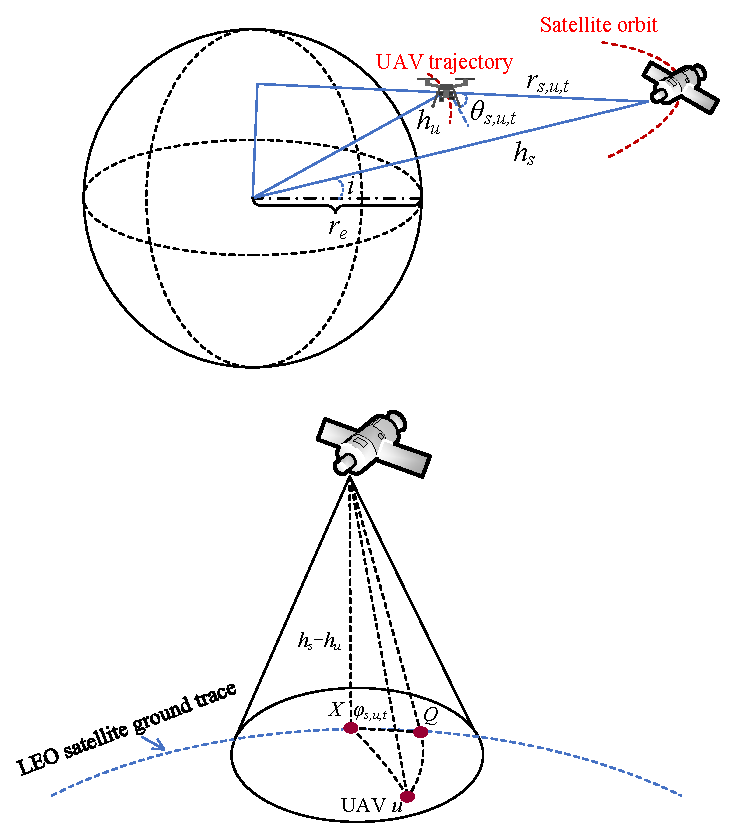
\includegraphics[width=0.95\columnwidth]{Definitions/figure2}
\caption{figure2.}
\label{fig2}
\end{figure}

A three-dimensional Cartesian coordinate system is employed to characterize the spatial locations of UAVs and IoT devices. The IoT devices are assumed to be randomly distributed on the ground plane, and the horizontal coordinate of the $k$-th device denoted as $\mathbf{q}_k = (x_k, y_k, 0)$. Each UAV operates at a fixed altitude $h_u$. Accordingly, the position of the $u$-th UAV at the $n$-th hover point is expressed as $\mathbf{q}_u(n) = (x_u(n), y_u(n), h_u)$. Due to the elevated UAV altitude and the unobstructed propagation environment, the wireless links between IoT devices and UAVs are dominated by line-of-sight (LoS) propagation. Under this condition, the channel gain between IoT device $k$ and its associated UAV is modeled as
\begin{quote}
\begin{equation}
G_k = \frac{\beta_0}{h_u^2 + (x_u(n) - x_k)^2 + (y_u(n) - y_k)^2},
\end{equation}
\end{quote}
where $\beta_0$ represents the channel gain at the reference distance $r_0$ = 1m.

Let $\mathcal{P}$ denote the set of all feasible transmission pairs, where each pair $p \in \mathcal{P}$ consists of either (i) two IoT devices forming a NOMA cluster or (ii) a single device operating in OFDMA mode. A binary decision variable $\delta_{p} \in \{0,1\}$ is introduced to indicate whether pair $p$ is activated. To ensure that each IoT device is assigned to at most one pair, the following constraint is imposed
\begin{quote}
\begin{equation}
\sum_{p \in P: k \in p} \delta_p \leq 1, \quad \forall k \in \mathcal{K}.
\end{equation}
\end{quote}

For an activated NOMA pair containing two devices $p = \{k, m\}$, the device with the stronger channel gain performs successive interference cancellation (SIC) and decodes the weaker device’s signal prior to decoding its own signal. The corresponding interference structure is determined by the activated pair $p$.

Given the pairing configuration, the received signal-to-interference-plus-noise ratio (SINR) of IoT device $k$ can be expressed as
\begin{quote}
\begin{equation}
\mathrm{SINR}_k = \frac{p_k G_k}{\sum_{\substack{p \in P \\ k,m \in p \\ m \neq k}} \delta_p p_m G_m + \sigma_{iu}^2},
\end{equation}
\end{quote}
where $p_k$ s the transmit power of device $k$, and $\sigma^2 _{iu}$ denotes the receiver noise power. Based on the obtained SINR, the achievable uplink data rate of device $k$ is
\begin{quote}
\begin{equation}
d_k = B_{iu} \log_2 \left(1 + \mathrm{SINR}_k\right),
\end{equation}
\end{quote}
where $B_{iu}$ represents the bandwidth allocated to UAV–IoT communications. Given the task data size $D_k$, the corresponding uplink transmission delay is
\begin{quote}
\begin{equation}
T_k^{{tr}} = \frac{D_k}{d_k},
\end{equation}
\end{quote}

A predetermined visiting order is assumed for each UAV to sequentially approach all NOMA groups and independent IoT devices after its trajectory has been determined. The trajectory of UAV $u$ is represented by the ordered set $\{\mathbf{q}_u(0), \mathbf{q}_u(1), \dots, \mathbf{q}_u(N_u)\}$, where $N_u$ denotes the number of hovering waypoints assigned to UAV $u$. Accordingly, the total flight path length of UAV $u$ over the entire mission is defined as
\begin{equation}
L_u = \sum_{n=0}^{N_u-1} \lVert \mathbf{q}_u(n+1) - \mathbf{q}_u(n) \rVert.
\end{equation}

Given a constant flight speed $v_f$, the required flight time for UAV $u$ is expressed as
\begin{equation}
T^{fly}_u = \frac{L_u}{v_f}.
\end{equation}

During the data collection phase, each UAV hovers at designated waypoints to receive data from IoT devices. The hovering duration of UAV $u$ is determined by the transmission times of all devices within the active pairs. Based on the pair-based NOMA definition, the hovering time is expressed as
\begin{equation}
T_u^{hov} = \sum_{p \in P} \delta_p \max_{k \in p} \frac{D_k}{d_k}.
\end{equation}

For NOMA pairs containing two devices, the maximum operator ensures that UAV $u$ hovers sufficiently long to receive the data from both devices in parallel, whereas for single-device OFDMA pairs, the expression reduces to the corresponding device’s transmission time.

The energy consumption of UAV $u$ in this phase comprises both hovering energy and flight-related energy. Accordingly, the total energy consumption of the UAV–IoT subsystem is
\begin{equation}
E_{total} = \sum_{u=1}^{U} (P_h T_u^{hov} + P_f T_u^{fly}),
\end{equation}
where $P_h$ and $P_f$ represent the hovering power and flight power of the UAVs, respectively, and $T^{fly}_u$ is the flight time of UAV $u$ as defined previously.

\subsection{Data Offloading from UAV to LEO}

After the UAV completes data collection from all IoT devices, it acquires the position information of all visible LEO satellites and selects the satellite that can satisfy the transmission demand. To represent the computation offloading decision, a binary association variable $\beta_{s,u,t} \in \{0, 1\}$ is introduced, where $\beta_{s,u,t} = 1$ indicates that UAV $u$ offloads its computation to satellite $s$ at time $t$. The channel gain between UAV $u$ and LEO satellite $s$ is modeled based on the free-space path loss as
\begin{equation}
G_{s,u,t}[dB] = 92.44 + 20\log_{10}(r_{s,u,t}) +20\log_{10}(f_s),
\end{equation}
where $f_s$ denotes the operating frequency of satellite $s$ in GHz, and $r_{s,u,t}$ is the straight-line distance between UAV $u$ and satellite $s$ at $t$. The distance $r_{s,u,t}$ is calculated according to the geometry of the Earth–UAV–satellite system
\begin{equation}
r_{s,u,t} = \sqrt{(r_e + h_s)^2 + (r_e + h_u)^2 - 2(r_e + h_s)(r_e + h_u) \cos \theta_{s,u,t}},
\end{equation}
where $r_e$ is the Earth radius, and $h_u$ and $h_s$ are the altitudes of the UAV and LEO satellite, respectively. The satellite elevation angle $\theta_{s,u,t}$ with respect to UAV $u$ according to \cite{seyedi2012trace} is computed as
\begin{equation}
\theta_{s,u,t} = \arctan \left( \frac{h_s - h_u}{d_{\mathrm{ground},s,u,t}} \right), \quad d_{\mathrm{ground},s,u,t} = r_e \phi_{s,u,t},
\end{equation}
where $d_{\mathrm{ground},s,u,t}$ is the horizontal distance on the Earth surface between UAV $u$ and the sub-satellite point of satellite $s$, and $\phi_{s,u,t}$ denotes the corresponding central angle on the Earth’s surface. The central angle $\phi_{s,u,t}$ varies over time according to the satellite and Earth motion
\begin{equation}
\phi_{s,u,t} = (\omega_E \cos i - \omega_S)(t - t_0) + \phi_{s,u,t_0},
\end{equation}
where $\omega_E$,  $\omega_S$ are the angular velocities of the Earth rotation and satellite orbit, $i$ is the orbital inclination of the satellite, $t_0$ is the time when the satellite becomes visible to the UAV, and $\phi_{s,u,t_0}$ is the initial central angle at $t_0$.

The received power at LEO satellite $s$ from UAV $u$ at time $t$ is expressed as
\begin{equation}
P_{s,u,t}^{re} = P_{tr} G_{tr} G_{re} G_{s,u,t}^{lin},
\end{equation}
where $P_{tr}$ denotes the transmit power of the UAV, $G_{tr}$ and $G_{re}$ are the transmit and receive antenna gains of the UAV and LEO satellite, respectively, and $G_{s,u,t}^{lin}$ is the linear-scale channel gain between UAV $u$ and satellite $s$, derived from the distance-dependent free-space path loss as described in subsection 2.1.

Based on the received power, the achievable uplink data rate from UAV $u$ to LEO satellite $s$ at time $t$ is calculated according to the Shannon capacity formula
\begin{equation}
d_{s,u,t} = B_{su} \log_2 \left(1 + \frac{P_{s,u,t}^{re}}{\sigma_{su}^2}\right),
\end{equation}
where $B_{su}$ denotes the available bandwidth of the UAV–LEO link, and $\sigma_{su}^2$ is the noise power at the satellite receiver. Let $x_{s,u,t} \in \{0,1\}$ represent the satellite association decision, where $x_{s,u,t} = 1$ indicates that UAV $u$ connects to satellite $s$ at time $t$.To characterize unnecessary switching, the handover indicator is defined as
\begin{equation}
 h_{u,t} = \frac{1}{2} \sum_{s=1}^{S} |x_{s,u,t} - x_{s,u,t-1}|.
\end{equation}

\subsection{Problem Formulation}

To minimize the total energy consumption of the first-stage IoT–UAV data collection process, the optimization is performed over the pair-based association variables $\boldsymbol{\delta} = \{\delta_p \mid p \in P\}$, the transmit power allocation of IoT devices $\mathbf{p} = \{p_k \mid k \in K\}$, and the UAV hovering positions and visiting order $\mathbf{q} = \{\mathbf{q}_u(n) \mid u \in U\}$. By jointly optimizing $\boldsymbol{\delta}$, $\mathbf{p}$, and $\mathbf{q}$, , the total UAV energy consumption consisting of hovering and flight energy is minimized. The optimization problem is detailed as
\begin{subequations}
\begin{align}
\mathcal{P}_1: \min_{\delta, \mathbf{p}, \mathbf{q}} \quad & 
\sum_{u=1}^{U} \left( P_h \sum_{p \in P_u} \delta_p \max_{k \in p} \frac{D_k}{d_k} + P_f \frac{L_u}{v_f} \right) \\
\text{s.t.} \quad & p_{\min} \leq p_k \leq p_{\max}, \quad \forall k, \label{eq:p1_power} \\
& \sum_{p: k \in p} \delta_p \leq 1, \quad \forall k, \label{eq:p1_assignment} \\
& \rho p_{i(p)} G_{i(p)} \leq p_{j(p)} G_{j(p)}, \quad \forall p \in P_{\text{NOMA}}, \label{eq:p1_noma} \\
& \mathbf{q}_u(N_u) = \mathbf{q}_u(0), \quad \forall u, \label{eq:p1_trajectory} \\
& \delta_p \in \{0, 1\}, \quad \forall p \in P. \label{eq:p1_binary}
\end{align}
\end{subequations}

Constraint \ref{eq:p1_power} restricts the transmit power of each IoT device within its allowable operating range. Constraint  \ref{eq:p1_assignment} ensures that each device can participate in at most one transmission group, thereby preventing conflicting pair assignments. Constraint \ref{eq:p1_noma} enforces the power-domain separation required for successful NOMA decoding in every selected NOMA pair, where $\rho \in (0,1)$ denotes the minimum ratio ensuring the correct decoding order. Constraint \ref{eq:p1_trajectory} guarantees that each UAV completes a closed trajectory, returning to its initial hovering point after visiting all designated positions. Constraint \ref{eq:p1_binary} defines the binary nature of the group-selection variables.

Due to the coupling among the discrete pairing decisions $\delta_p$, the continuous transmit-power variables $\{p_k\}$, and the UAV trajectory variables $\mathbf{q}_u(n)$, the overall optimization problem P1 forms a mixed-integer nonlinear programming model, which is NP-hard and computationally intractable to solve optimally.

After completing the IoT data-collection stage, the UAV proceeds to offload its aggregated task data to LEO satellites. The primary objective of the second-stage satellite association problem is to minimize unnecessary handover frequency while meeting operational offloading requirements, thereby enhancing QoS assurance and indirectly reducing both transmission energy consumption and handover energy consumption for unmanned aerial vehicles.

Demand-Aware  Handover does not seek to solve an optimal global objective function, but rather proposes a strategy algorithm that satisfies the following constraints
\begin{subequations}
\begin{align}
\mathcal{P}_2: \min \quad & 
\sum_{u=1}^{U} \sum_{t=1}^{T} h_{u,t} \\
\text{s.t.} \quad & \sum_{s=1}^{S} \sum_{t=1}^{T} x_{s,u,t} d_{s,u,t} \Delta t \geq D_u, \quad \label{eq:p2_total}\\
&\sum_{s=1}^{S} x_{s,u,t} \leq 1, \quad \forall t \in \mathcal{T}, \label{eq:p2_visible} \\
& \theta_{s,u,t} \geq \theta_{\min}, \quad \label{eq:p2_elevation} \\
& \sum_{s=1}^{S} \sum_{t'=t}^{T} x_{s,u,t'} d_{s,u,t'} \Delta t \geq D_u^{rem}(t). \label{eq:p2_remaining} 
\end{align}
\end{subequations}

Constraint \ref{eq:p2_total} represents the total amount of data successfully offloaded during the mission must satisfy $D_u$ is the task data size to be transmitted. Constraint \ref{eq:p2_visible} represents communication continuity requires that the UAV is associated with at most one visible satellite at any time. Constraint \ref{eq:p2_elevation} represents only satellites satisfying the minimum elevation constraint are eligible for association. Constraint \ref{eq:p2_remaining} ensures that switching is triggered only when the current satellite can no longer satisfy the remaining demand under predicted link evolution where $D_u^{rem}(t)$ denotes the remaining data to be uploaded at time $t$.

\section{ALGORITHM DESIGN}

The model is divided into two stages to achieve an effective solution. Specifically: during the data transmission phase from IoT devices to drones, Algorithm 1 completes IoT pairing, power allocation, and drone flight path planning; during the data transmission phase from drones to low-orbit satellites, Algorithm 2 selects link-demand-aware low-orbit satellites to ensure QoS.

\subsection{UAV Data Collection and Energy Optimization}

To effectively solve problem $\mathcal{P}_1$, the total energy consumption in the IoT-UAV phase is considered. Since the IoT transmission energy is negligible compared to UAV hovering and flight energy, the optimization focuses on minimizing the UAV energy consumption, which consists of hovering energy and flight energy. The problem involves coupled discrete pairing decisions $\delta = \{\delta_p | p \in \mathcal{P}\}$, continuous transmit power variables $\mathbf{p} = \{p_k | k \in \mathcal{K}\}$, and UAV hovering positions $\mathbf{q} = \{\mathbf{q}_u(n) | u \in \mathcal{U}\}$. This mixed-integer nonlinear programming problem is challenging to solve directly. Therefore, an algorithm framework based on alternating optimization and local search is proposed, as illustrated in Fig.~\ref{fig:algorithm_flowchart} and detailed in Algorithm~1.

The initial NOMA pairs are constructed based on distance constraints. Specifically, the distance matrix among all IoT devices is computed, and NOMA pairs are formed by grouping the two nearest devices that satisfy the pairing constraint into the pair set $\mathcal{P}$. This process repeats until no new valid pairs can be formed, and the remaining devices operate as independent OFDMA nodes.

For each activated pair $p \in \mathcal{P}$ with $\delta_p = 1$, an alternating optimization strategy is adopted to jointly optimize power allocation and hovering positions. Given fixed UAV hovering position $(x_u, y_u, h_u)$, the transmit powers of paired devices are iteratively updated using Newton's method. For a NOMA pair $p = \{k, m\}$, $p_m$ is alternately updated while fixing $p_k$ and vice versa until convergence. For independent OFDMA nodes, $p_k = p_{\max}$ is directly set to maximize throughput.

Given fixed power allocation, the UAV hovering position $(x_u, y_u)$ (with altitude $h_u$ kept fixed) is optimized using the Adam optimizer. Unlike gradient-free methods, Adam leverages adaptive learning rates and momentum to achieve faster convergence and finer position adjustments. The position update rule is given by:
\begin{align}
\mathbf{m}_t &= \beta_1 \mathbf{m}_{t-1} + (1-\beta_1)\nabla_{\mathbf{q}} E_{\text{total}}, \\
\mathbf{v}_t &= \beta_2 \mathbf{v}_{t-1} + (1-\beta_2)(\nabla_{\mathbf{q}} E_{\text{total}})^2, \\
\mathbf{q}_u^{(t+1)} &= \mathbf{q}_u^{(t)} - \alpha \frac{\hat{\mathbf{m}}_t}{\sqrt{\hat{\mathbf{v}}_t} + \epsilon},
\end{align}
where $\mathbf{m}_t$ and $\mathbf{v}_t$ are the first and second moment estimates, $\alpha$ is the learning rate, and $\beta_1, \beta_2$ are decay rates. The alternating optimization process iterates until reaching the maximum iteration count $J$ or until the objective function change falls below a threshold.

After obtaining all hovering positions, the UAV visiting order must be planned to minimize flight distance. This problem is essentially a variant of the multiple traveling salesman problem (mTSP). The 2-opt local search algorithm is employed for trajectory optimization. The 2-opt algorithm iteratively removes two edges from the trajectory and reconnects them to eliminate path crossings, thereby progressively improving solution quality until reaching a local optimum. Compared to metaheuristic methods, 2-opt provides faster convergence and more stable performance for trajectory optimization.

To further reduce energy consumption, a pair recombination mechanism is introduced. All unpaired nodes are traversed to check if there exist opportunities to recombine with existing paired nodes. If an unpaired node is closer to one member of an existing pair, the original pair is broken and a new NOMA pair is formed. For two spatially close NOMA pairs, their members are exchanged to reduce UAV flight distance or hovering time.

After each recombination or exchange operation, the UAV trajectory and total energy consumption are recalculated. The new configuration is accepted if it yields lower energy consumption; otherwise, the original configuration is retained. Through multiple rounds of exchange operations, the algorithm can escape local optima and obtain better NOMA pairing schemes. The complete algorithm flow is presented in Algorithm~1 with the corresponding flowchart shown in Fig.~\ref{fig:algorithm_flowchart}.

\begin{figure*}[!t]
\centering
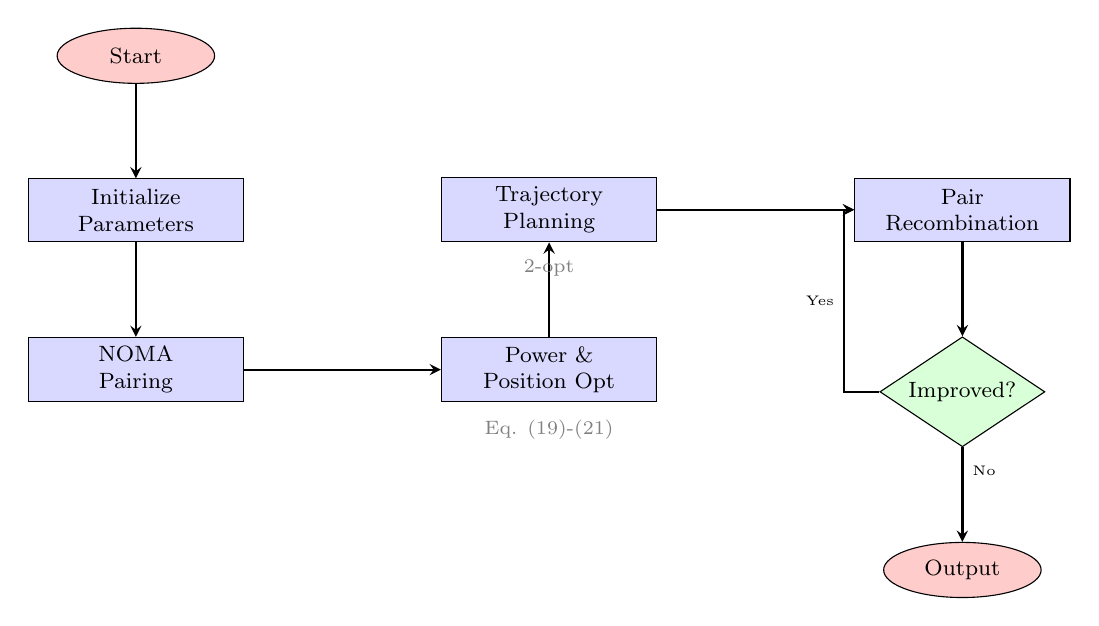
\begin{tikzpicture}[
    node distance=1.2cm and 2.5cm,
    startstop/.style={ellipse, draw, fill=red!20, text centered, minimum height=0.7cm, minimum width=2cm, font=\footnotesize},
    process/.style={rectangle, draw, fill=blue!15, text centered, text width=2.5cm, minimum height=0.8cm, font=\footnotesize},
    decision/.style={diamond, draw, fill=green!15, text centered, minimum height=1cm, minimum width=1cm, aspect=1.5, font=\footnotesize, inner sep=2pt},
    arrow/.style={thick,->,>=stealth}
]

% 第一列(从上到下)
\node (start) [startstop] {Start};
\node (init) [process, below=of start] {Initialize\\Parameters};
\node (pairing) [process, below=of init] {NOMA\\Pairing};

% 第二列(从下到上)
\node (optimization) [process, right=of pairing] {Power \&\\Position Opt};
\node (trajectory) [process, above=of optimization] {Trajectory\\Planning};

% 第三列(从上到下)
\node (exchange) [process, right=of trajectory] {Pair\\Recombination};
\node (check) [decision, below=of exchange] {Improved?};
\node (stop) [startstop, below=of check] {Output};

% 主流程箭头
\draw [arrow] (start) -- (init);
\draw [arrow] (init) -- (pairing);
\draw [arrow] (pairing) -- node[midway, below, font=\tiny] {} (optimization);
\draw [arrow] (optimization) -- (trajectory);
\draw [arrow] (trajectory) -- node[midway, below, font=\tiny] {} (exchange);
\draw [arrow] (exchange) -- (check);
\draw [arrow] (check) -- node[near start, right, font=\tiny] {No} (stop);

% 反馈循环:从check向左转弯再向上到exchange
\draw [arrow] (check) -- ++(-1.5,0) |- node[near start, left, font=\tiny] {Yes} (exchange);

% 可选:添加小注释框(使用虚线边框,放在节点下方)
\node[below=0.1cm of optimization, font=\scriptsize, text=gray] {Eq. (19)-(21)};
\node[below=0.1cm of trajectory, font=\scriptsize, text=gray] {2-opt};

\end{tikzpicture}
\caption{Flowchart of the proposed algorithm for UAV data collection and energy optimization.}
\label{fig:algorithm_flowchart}
\end{figure*}

\begin{algorithm}
\caption{UAV Data Collection and Energy Optimization}
\label{alg:p1_optimization}
\begin{algorithmic}[1]
\State \textbf{Input:} All IoT devices' positions $\mathbf{q}_k$ and corresponding packets $D_k$, UAV initial position $\mathbf{q}_u(0)$
\State \textbf{Output:} Energy consumption $E_{\text{total}}$
\State Initialize distance matrix and maximum iterations $J$
\State Form NOMA pairs from two nearest devices under distance constraints
\State Obtain lists of paired and unpaired nodes
\For{each paired nodes $(k, m)$}
    \State Initialize transmission powers $p_k, p_m$
    \State Initialize hover position $(x_u, y_u, h_u)$
    \State Set iteration counter $j \leftarrow 0$
    \While{$j \leq J$}
        \State Update $p_k^{(j)}, p_m^{(j)}$ using Newton's method
        \State Update $(x_u^{(j)}, y_u^{(j)}, h_u)$ using Adam optimizer
        \State $j \leftarrow j + 1$
    \EndWhile
\EndFor
\State Optimize UAV trajectories using 2-opt local search
\State Compute energy consumption $E_{\text{total}}$ using Eq.~(9)
\For{each node combination (unpaired and paired)}
    \State Exchange nodes between paired and unpaired groups
    \State Update UAV trajectories and device transmission powers
    \State Calculate new energy consumption $E_{\text{new}}$ using Eq.~(9)
    \If{$E_{\text{new}} < E_{\text{total}}$}
        \State $E_{\text{total}} \leftarrow E_{\text{new}}$
    \EndIf
\EndFor
\State \Return $E_{\text{total}}$
\end{algorithmic}
\end{algorithm}

\subsection{LEO Satellite Selection Optimization}

After the UAV completes data collection from all IoT devices, it must offload the aggregated data to LEO satellites for further processing. Unlike static ground stations, LEO satellites exhibit high mobility with time-varying channel conditions and limited visibility windows. Consequently, the satellite association decision directly impacts both transmission efficiency and handover frequency.Frequent satellite handovers introduce signaling overhead, packet loss, and interruption delays, degrading quality of service. Conversely, maintaining connection with a suboptimal satellite prolongs transmission time and increases energy consumption. Therefore, the selection strategy must balance handover frequency against link quality to ensure timely and reliable data offloading.

To address problem P2, a demand-aware satellite selection mechanism is proposed. Rather than myopically selecting the satellite with maximum instantaneous throughput at each time slot, the algorithm evaluates whether the current satellite can satisfy the remaining data transmission demand under predicted link evolution. Satellite handover is triggered only when the current satellite is predicted to be insufficient for completing the remaining task, thereby minimizing unnecessary switching while ensuring transmission deadlines.


The algorithm operates as follows. At each decision epoch, all LEO satellites satisfying the elevation angle constraint $\theta_{s,u,t} \geq \theta_{\min}$ are identified as candidate satellites. For each candidate $s$, the instantaneous uplink data rate $d_{s,u,t}$ is calculated according to Eq. (15) based on the distance-dependent channel gain and transmit power. The algorithm then predicts the cumulative throughput achievable by the current satellite over the remaining visibility window. If the predicted throughput exceeds the remaining data size $D_u^{\text{rem}}(t)$, the current satellite association is maintained. Otherwise, the algorithm selects the satellite with maximum instantaneous throughput from the candidate set and performs handover.

\begin{algorithm}[ht]
\caption{Demand-Aware LEO Satellite Selection}
\label{alg:satellite_selection}
\begin{algorithmic}[1]
\State \textbf{Input:} UAV position $\mathbf{q}_u(t)$, total data size $D_u$, transmitted data $D_u^{\text{tx}}$, current satellite $s_{\text{curr}}$, time $t$, prediction horizon $\Delta t$
\State \textbf{Output:} Selected satellite $s^*$
\State Compute remaining data: $D_u^{\text{rem}}(t) \gets D_u - D_u^{\text{tx}}$
\State Initialize candidate set: $\mathcal{S}_{\text{candidate}} \gets \emptyset$
\For{each satellite $s \in \mathcal{S}$}
    \State Compute elevation angle $\theta_{s,u,t}$ using Eq.~(12)
    \If{$\theta_{s,u,t} \geq \theta_{\min}$}
        \State Add $s$ to $\mathcal{S}_{\text{candidate}}$
    \EndIf
\EndFor
\If{$s_{\text{curr}} \in \mathcal{S}_{\text{candidate}}$}
    \State Compute current throughput: $d_{s_{\text{curr}},u,t}$ using Eq.~(15)
    \State Predict remaining visibility time: $T_{\text{vis}} \gets T_{\text{access}}(s_{\text{curr}}) - t$
    \State Estimate achievable data: $\hat{D}_{\text{curr}} \gets d_{s_{\text{curr}},u,t} \cdot \min(T_{\text{vis}}, \Delta t)$
    \If{$\hat{D}_{\text{curr}} \geq D_u^{\text{rem}}(t)$}
        \State \Return $s_{\text{curr}}$ \Comment{Current satellite sufficient}
    \EndIf
\EndIf
\State $s^* \gets \arg\max_{s \in \mathcal{S}_{\text{candidate}}} d_{s,u,t}$ \Comment{Select maximum throughput satellite}
\State \Return $s^*$
\end{algorithmic}
\end{algorithm}

\begin{table}[!t]
\centering
\caption{SIMULATION PARAMETERS}
\label{tab:simulation_parameters}
\begin{tabular}{llll}
\toprule
\textbf{Parameter} & \textbf{Value} & \textbf{Parameter} & \textbf{Value} \\
\midrule
$K$ (IoT devices) & 20 & $N$ (hover points) & 10 \\
$D_k$ (data size) & 10 MB & $B_{iu}$ & 1 MHz \\
$P_{\max}$ & 5 W & $P_{\min}$ & 0.1 W \\
$P_h$ & 100 W & $P_f$ & 150 W \\
$v_f$ & 10 m/s & $h_u$ & 100 m \\
$\beta_0$ & $10^{-5}$ & $\sigma^2_{iu}$ & $10^{-9}$ W \\
$\rho$ & 0.8 & $d_{\max}$ & 100 m \\
Area size & $500 \times 500$ m$^2$ & $\alpha$ (Adam) & 0.01 \\
$\beta_1$ (Adam) & 0.9 & $\beta_2$ (Adam) & 0.999 \\
$J$ (max iterations) & 100 & $\epsilon$ & $10^{-6}$ \\
\bottomrule
\end{tabular}
\end{table}

\begin{table}[!t]
\centering
\caption{LEO SATELLITE PARAMETERS}
\label{tab:leo_parameters}
\begin{tabular}{llll}
\toprule
\textbf{Parameter} & \textbf{Value} & \textbf{Parameter} & \textbf{Value} \\
\midrule
$\theta_{\min}$ & 15$^\circ$ & $B_{su}$ & 10 MHz \\
$P_{tr}$ & 10 W & $G_{tr}$ & 10 dBi \\
$G_{re}$ & 30 dBi & $\sigma^2_{su}$ & $4 \times 10^{-14}$ W \\
$f_s$ & 20 GHz & $r_e$ & 6378 km \\
$h_s$ (LEO altitude) & 550 km & $\omega_E$ & 7.29 rad/s \\
Constellation & Starlink & Num. satellites & 200 \\
\bottomrule
\end{tabular}
\end{table}
%%%%%%%%%%%%%%%%%%%%%%%%%%%%%%%%%%%%%%%%%%
\section{SIMULATION RESULTS}

This section evaluates the performance of our proposed two-stage optimization framework for UAV-assisted IoT data collection and LEO satellite offloading in SAGIN. We begin by presenting the simulation setup for both algorithms, followed by comprehensive performance analyses that demonstrate the effectiveness of each stage. The evaluation encompasses not only individual algorithm performance but also the synergistic effects of the end-to-end system.
\subsection{Simulation Setup}

Our evaluation framework is designed to assess a complete data collection and offloading mission in SAGIN, where ground IoT devices transmit data to UAVs (Stage 1), and UAVs subsequently offload the aggregated data to LEO satellites for cloud processing (Stage 2). All simulations are implemented in Python 3.10 and executed on a workstation equipped with an Intel Core i7-12700K processor and 32GB RAM.

The first stage focuses on the ground-to-air segment, where UAVs must efficiently collect data from spatially distributed IoT devices while minimizing energy consumption. We consider a square coverage area of $500\,\text{m} \times 500\,\text{m}$ containing $K$ IoT devices, where $K$ varies from 20 to 50 to evaluate scalability. Three UAVs operate at a fixed altitude of 100~m with a maximum transmit power of 0.1~W per device. The communication channel is modeled with a bandwidth of 1~MHz and noise power spectral density of $-174$~dBm/Hz. The path loss exponent is set to 2.5, representing typical urban propagation environments. To ensure statistical reliability, each configuration is evaluated across three different random seeds (27, 37, 41), and results are averaged. The UAV hovering power and flight power are set to $P_h = 80$~W and $P_f = 120$~W, respectively, based on typical small UAV specifications.

To benchmark the proposed Algorithm 1, we compare against three baseline methods representing different optimization strategies. The \textit{Random Pairing} baseline randomly groups IoT devices into NOMA pairs without considering spatial proximity or channel conditions, establishing a lower bound on achievable performance. The \textit{Fixed Hovering} method employs a greedy strategy that maximizes hovering time at each service point but neglects trajectory optimization, resulting in potentially long flight distances. The \textit{Basic Optimization} approach incorporates NOMA pairing, power allocation, and position optimization but lacks the advanced trajectory refinement of our proposed method. Our \textit{Proposed Method} (denoted as Adam-2opt) builds upon Basic Optimization by integrating the Adam optimizer for hovering position refinement and applying 2-opt local search for trajectory optimization.

The second stage addresses the air-to-space segment, where UAVs must maintain stable connectivity with rapidly moving LEO satellites. We simulate the Starlink constellation at an altitude of 550~km, with the number of visible satellites varying from 500 to over 1500 depending on the time window. The UAV is positioned at $(15^\circ\text{N}, 118^\circ\text{E})$ at an altitude of 200~m, using a carrier frequency of 20~GHz and channel bandwidth of 10~MHz. The minimum elevation angle is constrained to $\theta_{\min} = 10^\circ$ to ensure acceptable link quality. Each handover incurs a 400~ms delay during which no data transmission occurs, representing realistic RF reconfiguration and protocol negotiation overhead. The simulation duration spans 10 minutes with a time step of 20 seconds, allowing us to observe multiple satellite passes and handover events. The demand rate is configured to 8~Mbps, corresponding to a typical 1080p video streaming application that represents moderate data offloading requirements.

We compare our proposed \textit{Demand-Aware} handover strategy against a conventional \textit{Greedy} approach. The Greedy method continuously seeks the satellite offering maximum instantaneous data rate, switching whenever a better candidate becomes visible. This strategy maximizes throughput but potentially causes frequent handovers and service interruptions. In contrast, our Demand-Aware method maintains the current satellite connection as long as it can satisfy the remaining data transmission requirements, switching only when necessary to meet the offloading deadline. This philosophy prioritizes connection stability and quality of service over peak throughput maximization.

\subsection{Performance of IoT-UAV Data Collection Stage}

The IoT-UAV data collection stage presents a challenging mixed-integer nonlinear programming problem involving coupled decisions on device pairing, power allocation, and UAV trajectory planning. Fig.~\ref{fig:comparison_4algorithms} presents a comprehensive performance comparison across four key metrics: total UAV energy consumption, flight energy, flight distance, and hovering energy. These results reveal several critical insights into the effectiveness of our proposed optimization approach.

% Figure 1: Four-algorithm comparison
\begin{figure}[!t]
\centering
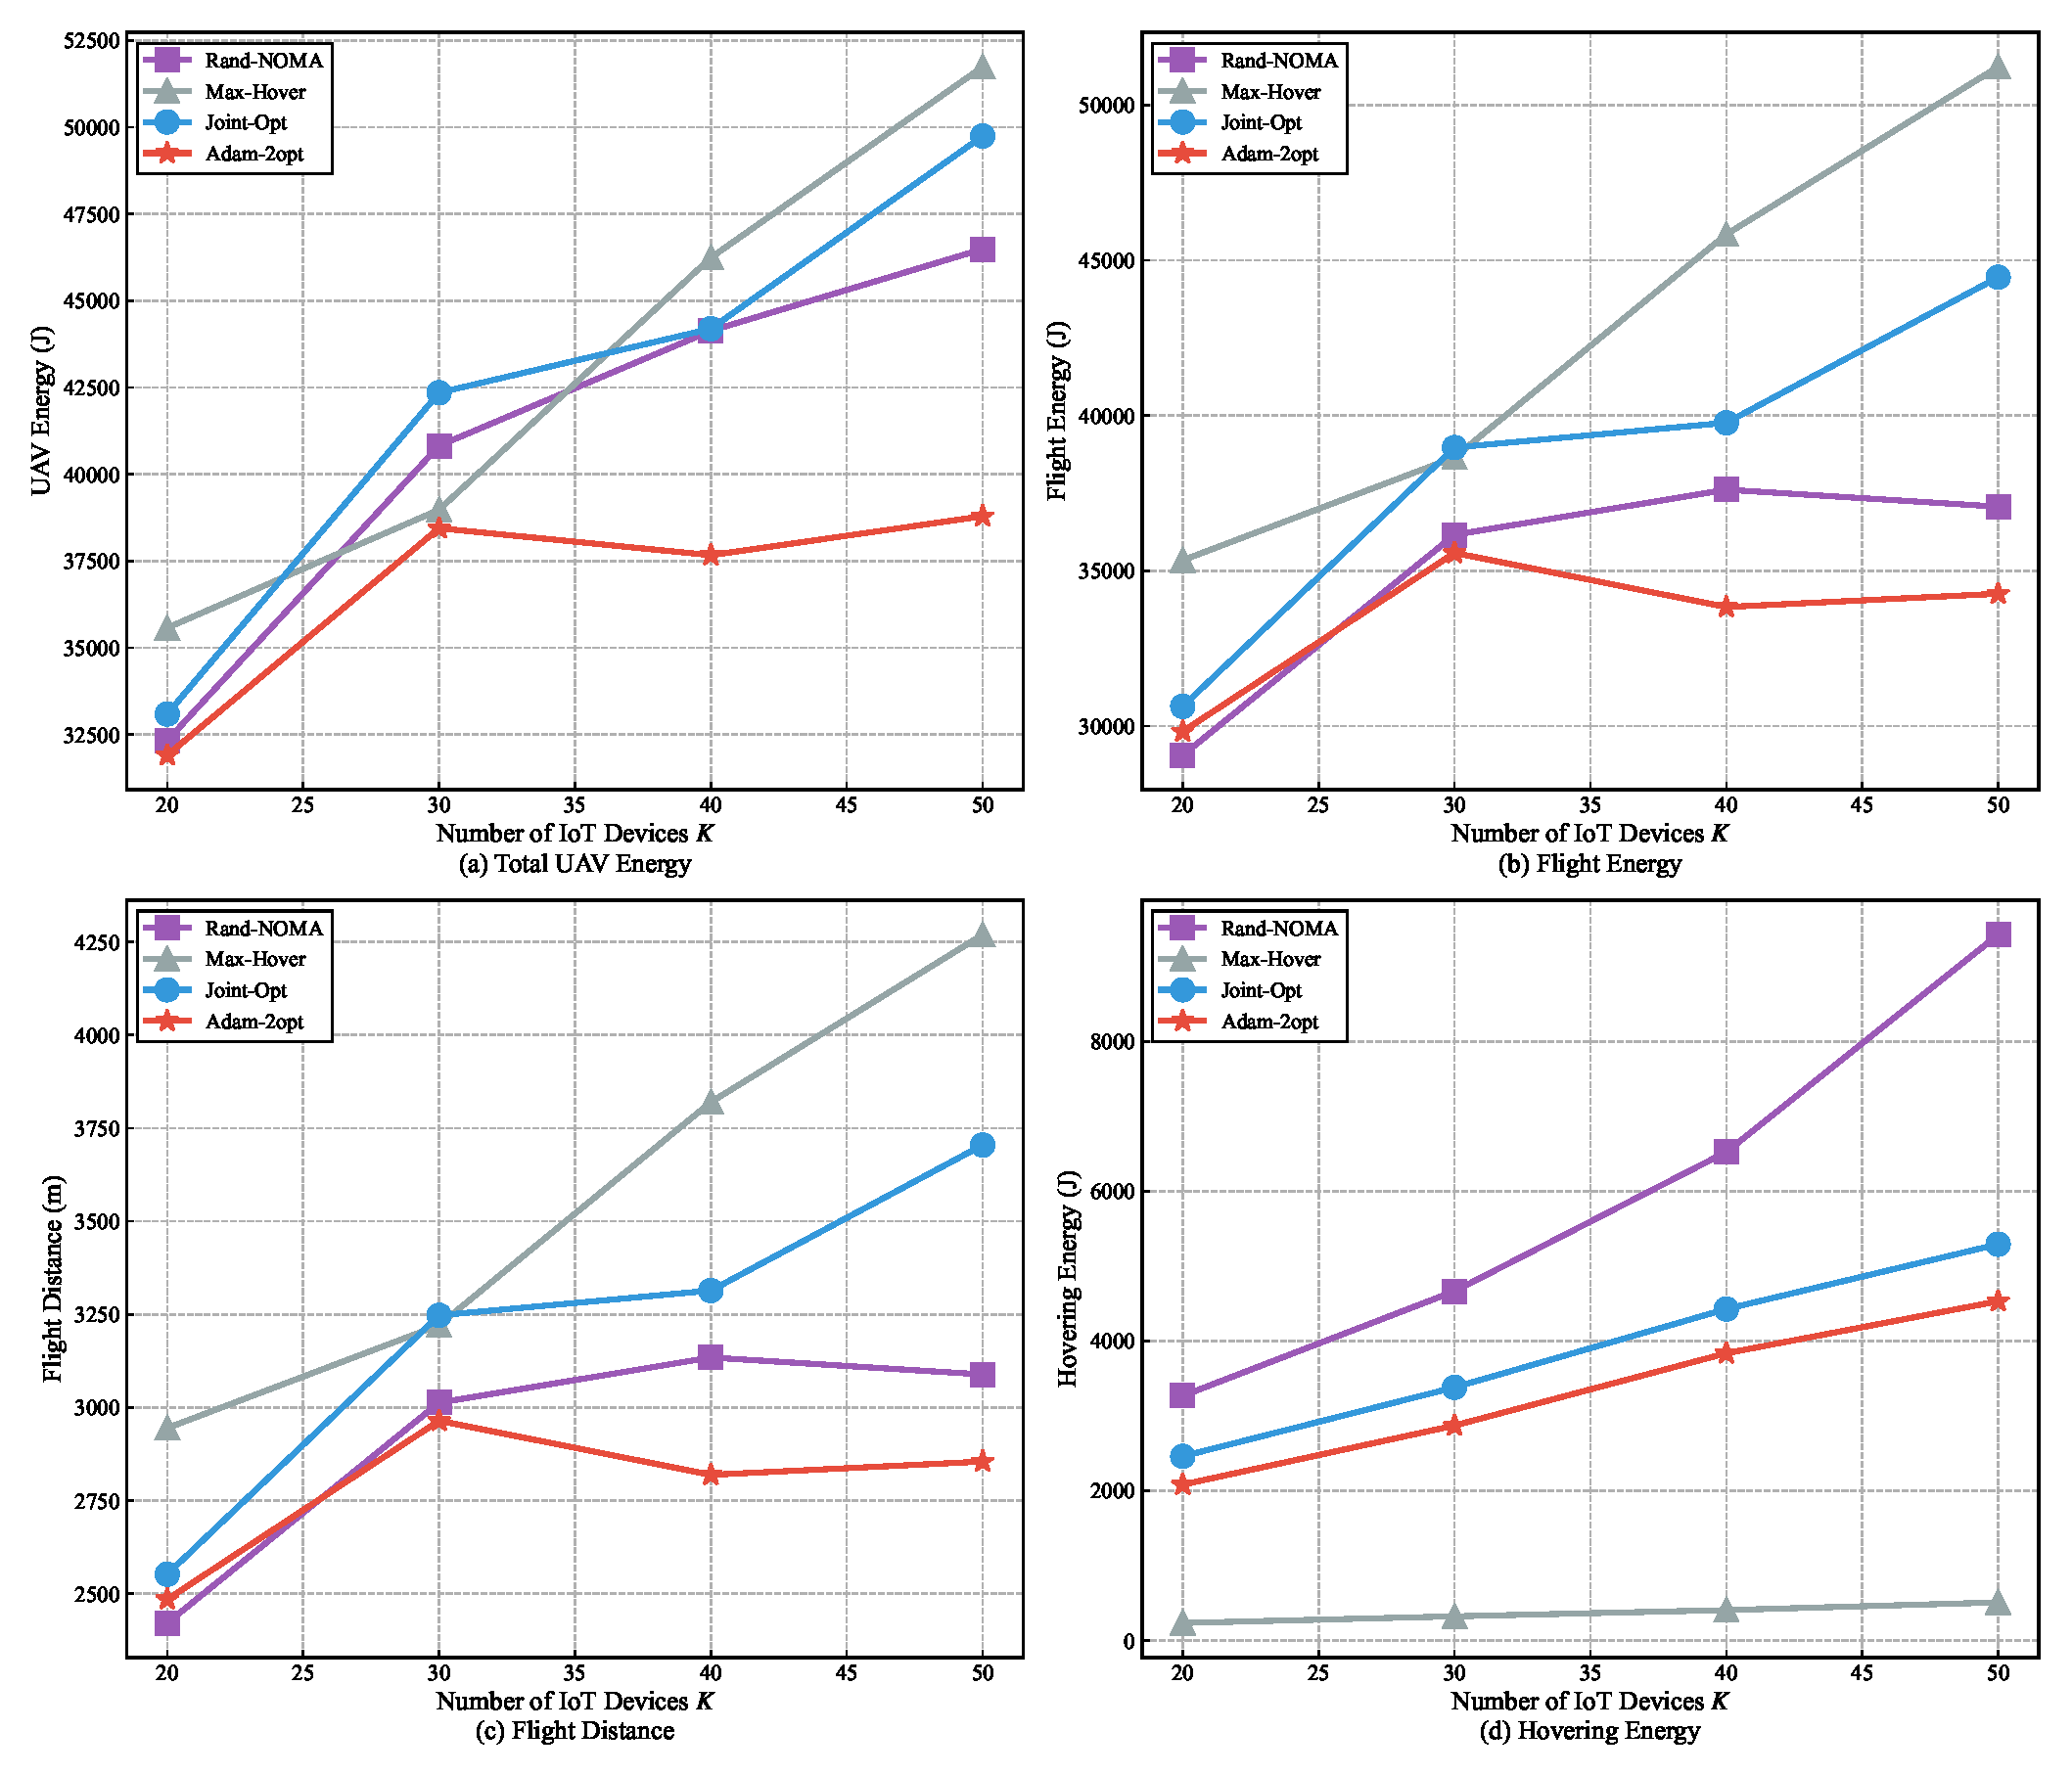
\includegraphics[width=0.95\columnwidth]{Definitions/comparison_4algorithms}
\caption{Performance comparison of four algorithms across varying numbers of IoT devices: (a) Total UAV energy consumption, (b) Flight energy, (c) Flight distance, and (d) Hovering energy. The proposed Adam-2opt method consistently achieves the lowest total energy consumption across all scenarios.}
\label{fig:comparison_4algorithms}
\end{figure}

Examining the total UAV energy consumption in Fig.~\ref{fig:comparison_4algorithms}(a), we observe that the proposed Adam-2opt algorithm consistently outperforms all baseline methods across the entire range of IoT device densities. For the most demanding scenario with $K=50$ devices, Adam-2opt achieves a total energy consumption of 38,789.84~J, representing a 16.6\% reduction compared to Random Pairing (46,490.88~J), a 25.0\% reduction compared to Fixed Hovering (51,741.77~J), and a 22.0\% reduction compared to Basic Optimization (49,747.93~J). The improvement becomes more pronounced as the network scales, with only 1.3\% energy savings at $K=20$ but expanding to 16.6\% at $K=50$. This trend indicates that the benefits of sophisticated trajectory optimization become increasingly significant in dense IoT deployments, where the complexity of visit sequencing and path planning grows substantially.

The superior energy performance of Adam-2opt stems from its effectiveness in both spatial dimensions of the optimization problem. Fig.~\ref{fig:comparison_4algorithms}(c) demonstrates that our method achieves significantly shorter flight distances compared to all baselines. At $K=50$, Adam-2opt requires only 2,854.92~m of flight distance, which is 7.6\% shorter than Random Pairing (3,088.77~m), 21.9\% shorter than Basic Optimization (3,704.63~m), and 33.1\% shorter than Fixed Hovering (4,269.38~m). The 2-opt local search algorithm plays a crucial role here by systematically eliminating trajectory crossings and unnecessary detours. This trajectory refinement not only reduces flight distance but also decreases flight energy proportionally, as evidenced in Fig.~\ref{fig:comparison_4algorithms}(b), where Adam-2opt consumes 34,259.07~J of flight energy compared to 37,065.30~J for Random Pairing and 51,232.53~J for Fixed Hovering.

An interesting observation emerges when examining the hovering energy patterns in Fig.~\ref{fig:comparison_4algorithms}(d). Fixed Hovering exhibits the lowest hovering energy (509.25~J at $K=50$) by design, as it minimizes the time spent at each service location. However, this strategy forces UAVs to traverse longer distances between widely separated service points, resulting in the highest total energy consumption. This demonstrates a fundamental trade-off in UAV mission planning: minimizing hovering time alone is insufficient if it leads to excessive flight distance. The Random Pairing baseline suffers from the opposite problem, with hovering energy of 9,425.58~J at $K=50$---more than double that of Adam-2opt (4,531.19~J). This inefficiency arises from suboptimal device pairing that creates geographically dispersed clusters, forcing UAVs to hover longer to serve poorly matched NOMA pairs. Our proposed method strikes an optimal balance, achieving 51.9\% hovering energy reduction compared to Random Pairing while simultaneously maintaining minimal flight distance.

To better understand the spatial efficiency of each algorithm, Fig.~\ref{fig:trajectory_comparison} visualizes the actual UAV trajectories for a representative scenario with $K=50$ devices. The visual comparison starkly illustrates the limitations of baseline approaches and the advantages of our optimization framework. The Random Pairing trajectory in Fig.~\ref{fig:trajectory_comparison}(a) exhibits numerous inefficiencies: UAV paths cross multiple times, backtracking occurs frequently, and the hovering points are distributed without clear spatial logic. This chaotic pattern reflects the arbitrary pairing decisions that ignore geographical proximity. The trajectory spans 3,509~m with 29 hovering points serving 21 paired devices, indicating substantial wasted motion.

% Figure 2: Trajectory comparison
\begin{figure*}[!t]
\centering
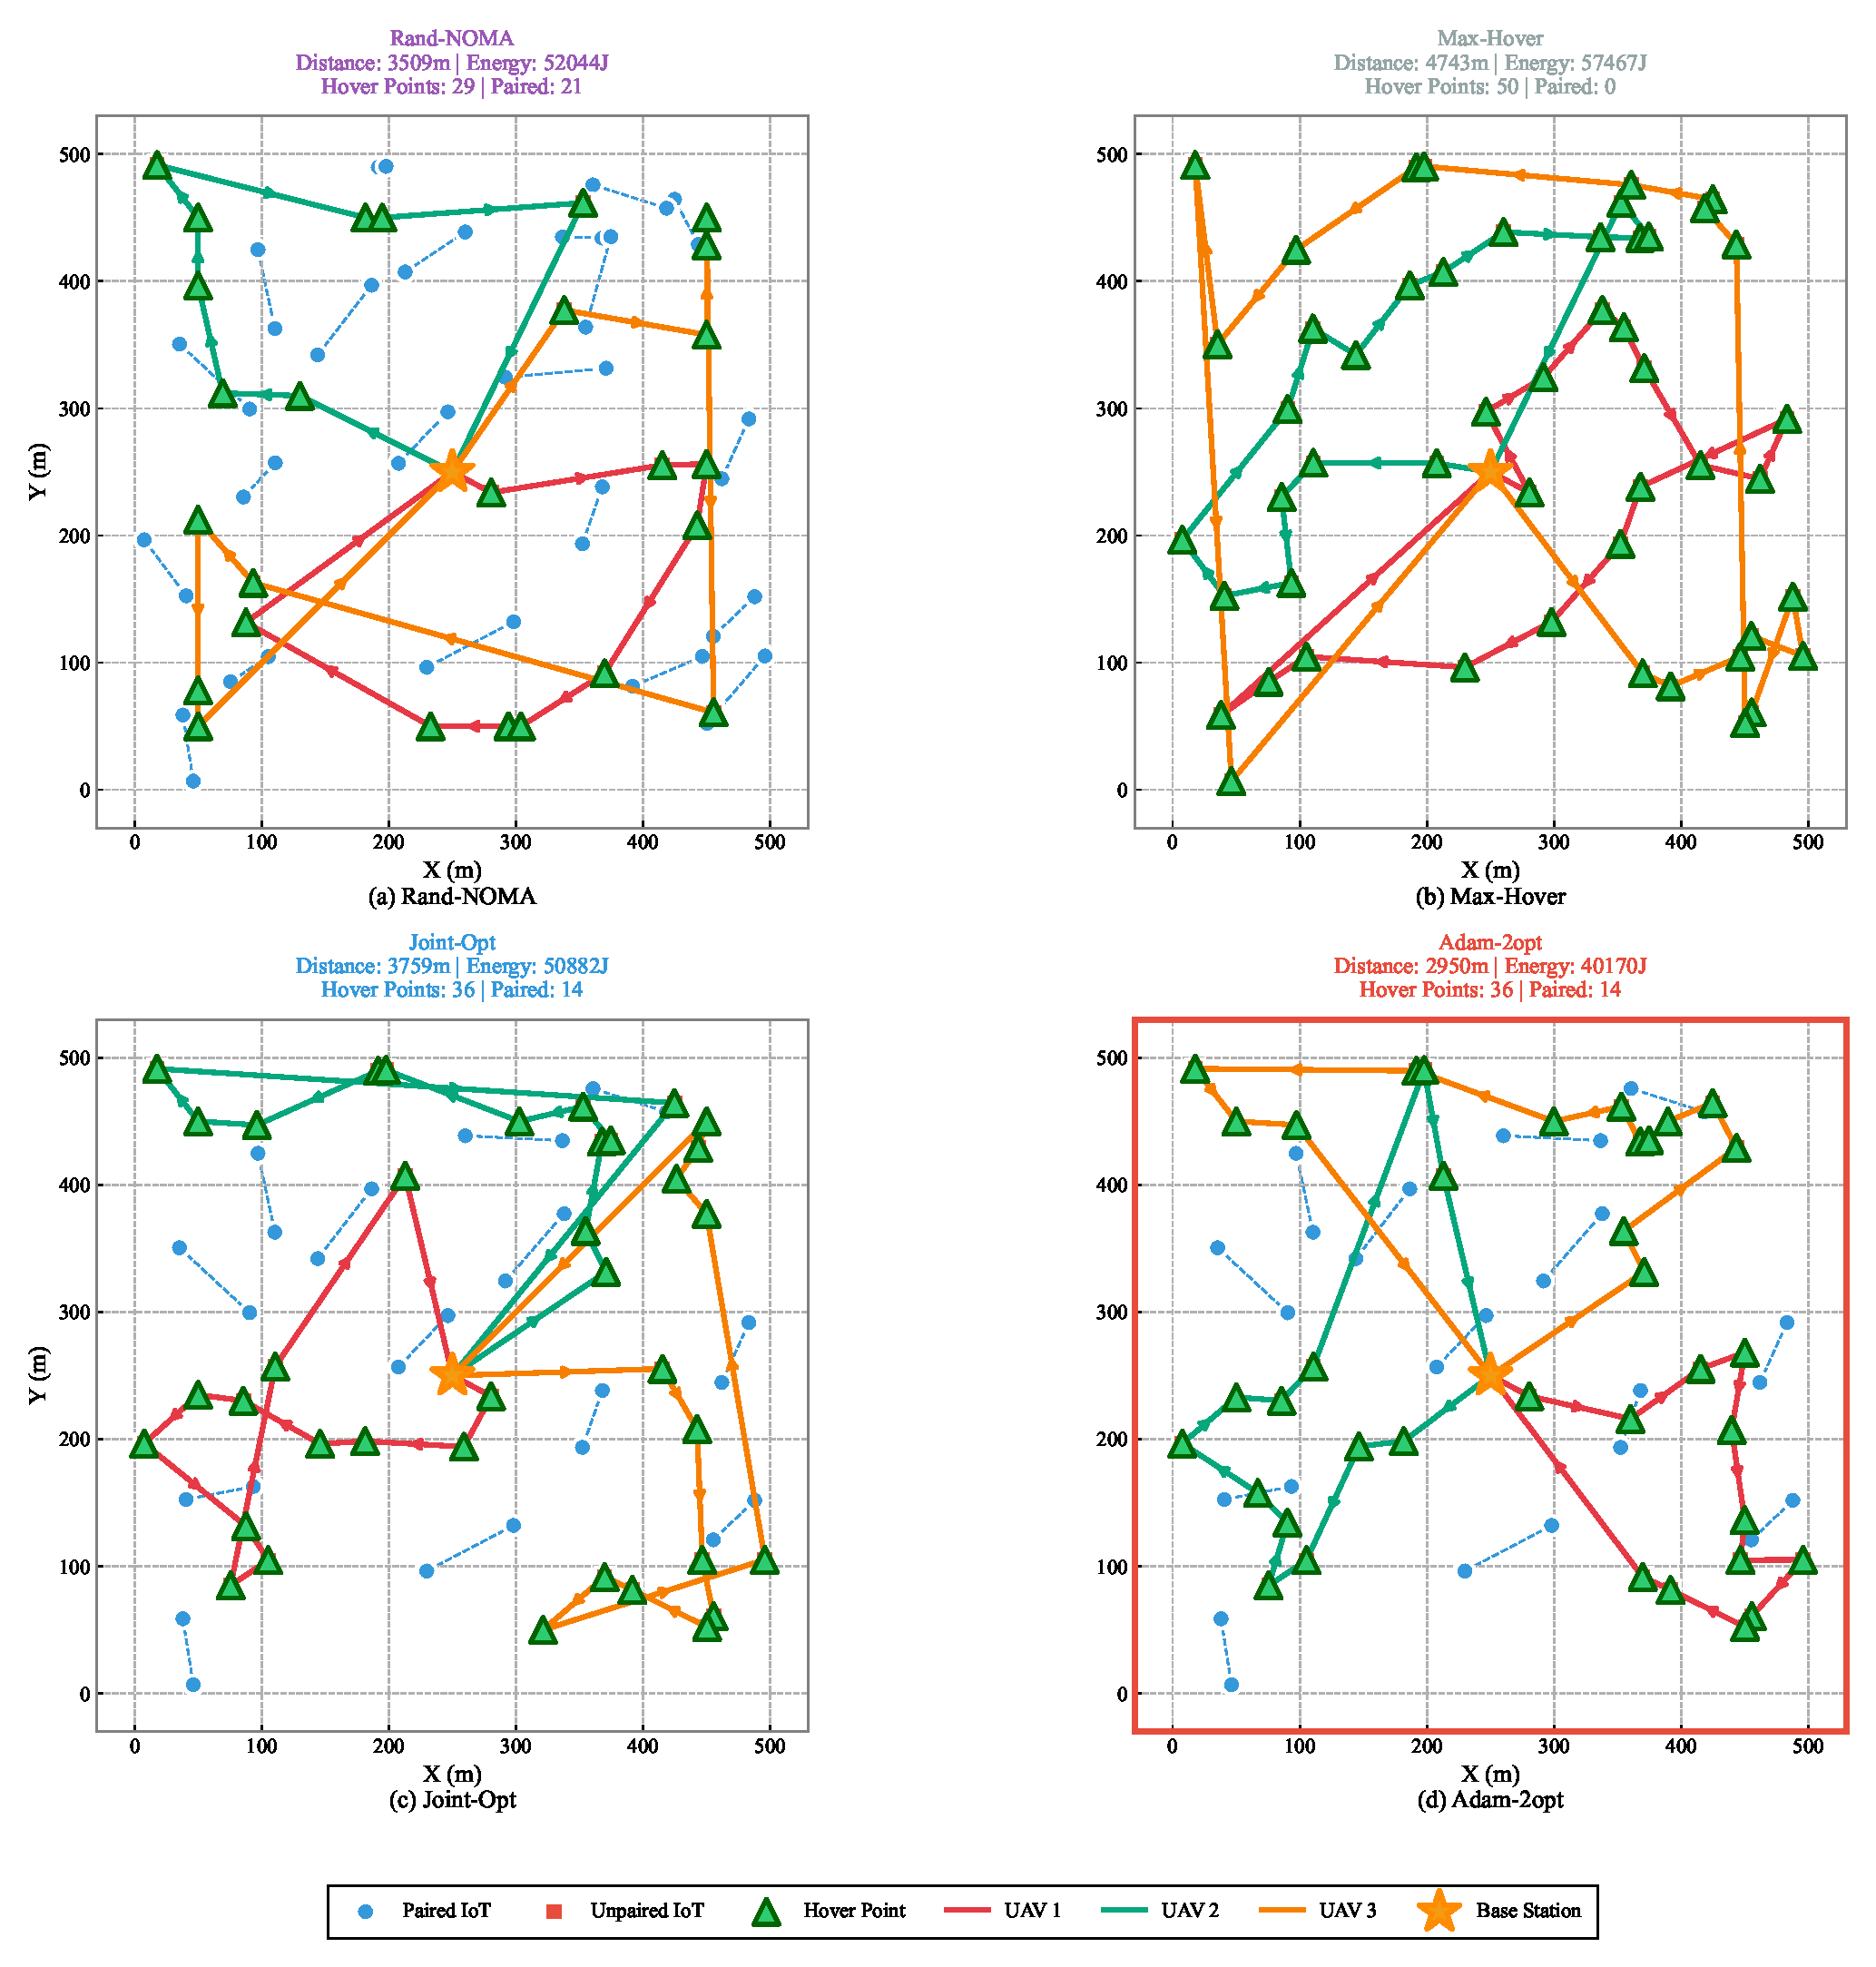
\includegraphics[width=0.95\textwidth]{Definitions/trajectory_comparison_4algorithms}
\caption{Trajectory visualization comparison for four algorithms ($K=50$ devices, seed 27): (a) Random Pairing exhibits random hovering point placement with multiple trajectory crossings, (b) Fixed Hovering creates extended flight paths due to predetermined service locations, (c) Basic Optimization shows improved hovering point placement through position optimization, and (d) Adam-2opt (Proposed) demonstrates the shortest and most efficient trajectories with eliminated crossings and optimal hovering point distribution.}
\label{fig:trajectory_comparison}
\end{figure*}

The Fixed Hovering approach in Fig.~\ref{fig:trajectory_comparison}(b) presents a different pathology. While the hovering points are well-distributed across the coverage area (50 points to ensure comprehensive coverage), the predetermined nature of these locations forces UAVs to visit many unnecessary waypoints. The resulting trajectory is remarkably long (4,743~m), with extensive empty flight segments between service clusters. This inflexibility in hovering point placement represents a fundamental flaw: maximizing hover point density does not translate to mission efficiency when device locations are non-uniform.

Basic Optimization in Fig.~\ref{fig:trajectory_comparison}(c) shows noticeable improvement over the two baselines. The algorithm successfully optimizes hovering point positions to better match device clusters, reducing the trajectory length to 3,759~m. However, the trajectory still contains visible crossings and suboptimal turn sequences, indicating that position optimization alone is insufficient. The lack of trajectory-level refinement leaves opportunities for further improvement.

The proposed Adam-2opt method in Fig.~\ref{fig:trajectory_comparison}(d) exhibits the most efficient trajectory structure. The path is notably smoother, with minimal backtracking and no trajectory crossings. The 2-opt refinement has successfully reordered the visit sequence to create a more logical flow pattern, reducing the total trajectory length to 2,950~m---the shortest among all methods. Importantly, this is achieved with 36 hovering points serving 14 paired devices, demonstrating that our algorithm balances multiple objectives simultaneously. The trajectory forms a more circular pattern that efficiently covers the device distribution while minimizing redundant motion. Each segment serves a clear purpose, and the directional flow minimizes the angular changes that would otherwise consume additional flight time and energy.

Beyond the primary energy and distance metrics, the computational complexity of each algorithm warrants consideration for practical deployment scenarios. The Random Pairing method executes in merely 0.1064 seconds for $K=50$ devices, as it performs only simple pairing operations without optimization. Fixed Hovering completes even faster at 0.0045 seconds due to its predetermined hovering grid and greedy power allocation. Basic Optimization requires 0.0613 seconds, balancing computational overhead with optimization quality. The proposed Adam-2opt method incurs the highest computational cost at 1.2024 seconds, attributable to the iterative Adam optimization and 2-opt trajectory refinement. However, this overhead remains entirely acceptable for offline mission planning scenarios, where trajectories can be pre-computed before deployment. The 16.6\% energy savings achieved by Adam-2opt far outweigh the modest increase in planning time, especially considering that UAV battery capacity is the primary limiting factor in long-duration missions.

The scalability characteristics revealed in Fig.~\ref{fig:comparison_4algorithms} provide important insights for system design. At low device densities ($K=20$), all methods achieve relatively similar performance (within 11\% of each other), suggesting that sophisticated optimization is less critical when the problem complexity is limited. However, as the network scales to $K=50$, the performance gap widens dramatically. Fixed Hovering's energy consumption increases by 45\% from $K=20$ to $K=50$, while Adam-2opt increases by only 21.6\%. This superior scaling behavior indicates that our algorithm's benefits become more pronounced precisely when they are most needed---in large-scale IoT deployments. The sublinear growth in Adam-2opt's energy consumption suggests that the algorithm effectively exploits the spatial clustering opportunities that emerge in denser networks, grouping nearby devices into efficient service routes.

% ==============================================================================
% 4.3 Performance of UAV-LEO Offloading Stage
% ==============================================================================

\subsection{Performance of UAV-LEO Offloading Stage}

Having established that Algorithm 1 effectively minimizes UAV energy consumption during ground data collection, we now examine the second stage of the system: offloading the aggregated data from UAVs to LEO satellites. This stage introduces distinct challenges fundamentally different from those in the IoT-UAV segment. LEO satellites orbit at approximately 7~km/s, resulting in rapidly time-varying channel conditions and limited visibility windows typically lasting only a few minutes. While Algorithm 1 focuses on spatial optimization in a relatively static environment, Algorithm 2 must address temporal dynamics and maintain service continuity despite continuous satellite motion.

The primary challenge in this stage is not maximizing instantaneous throughput, but rather balancing throughput requirements with connection stability. Frequent satellite handovers degrade quality of service through packet loss during switching intervals, increased signaling overhead, and potential service interruptions. Our Demand-Aware strategy addresses this challenge by maintaining the current satellite connection as long as it satisfies the data offloading requirements, switching only when the predicted link quality becomes insufficient to complete the remaining transmission within the mission deadline.

Fig.~\ref{fig:demand_aware_satellites} illustrates the data rate evolution over a 10-minute observation window for both the Greedy and Demand-Aware strategies across three satellite density scenarios. The contrast in behavior is immediately apparent. The Greedy strategy exhibits highly volatile data rates with frequent fluctuations between peaks above 40~Mbps and valleys below 20~Mbps. The numerous handover markers (triangles for Greedy, squares for Demand-Aware) clustered throughout the timeline reveal aggressive switching behavior. In the 500-satellite scenario, Greedy performs 7 handovers, while in the full constellation scenario, this increases to 9 handovers. Each handover represents a potential service disruption and contributes to packet loss during the 400~ms switching interval.

% Figure 3: Data rate comparison
\begin{figure*}[!t]
\centering
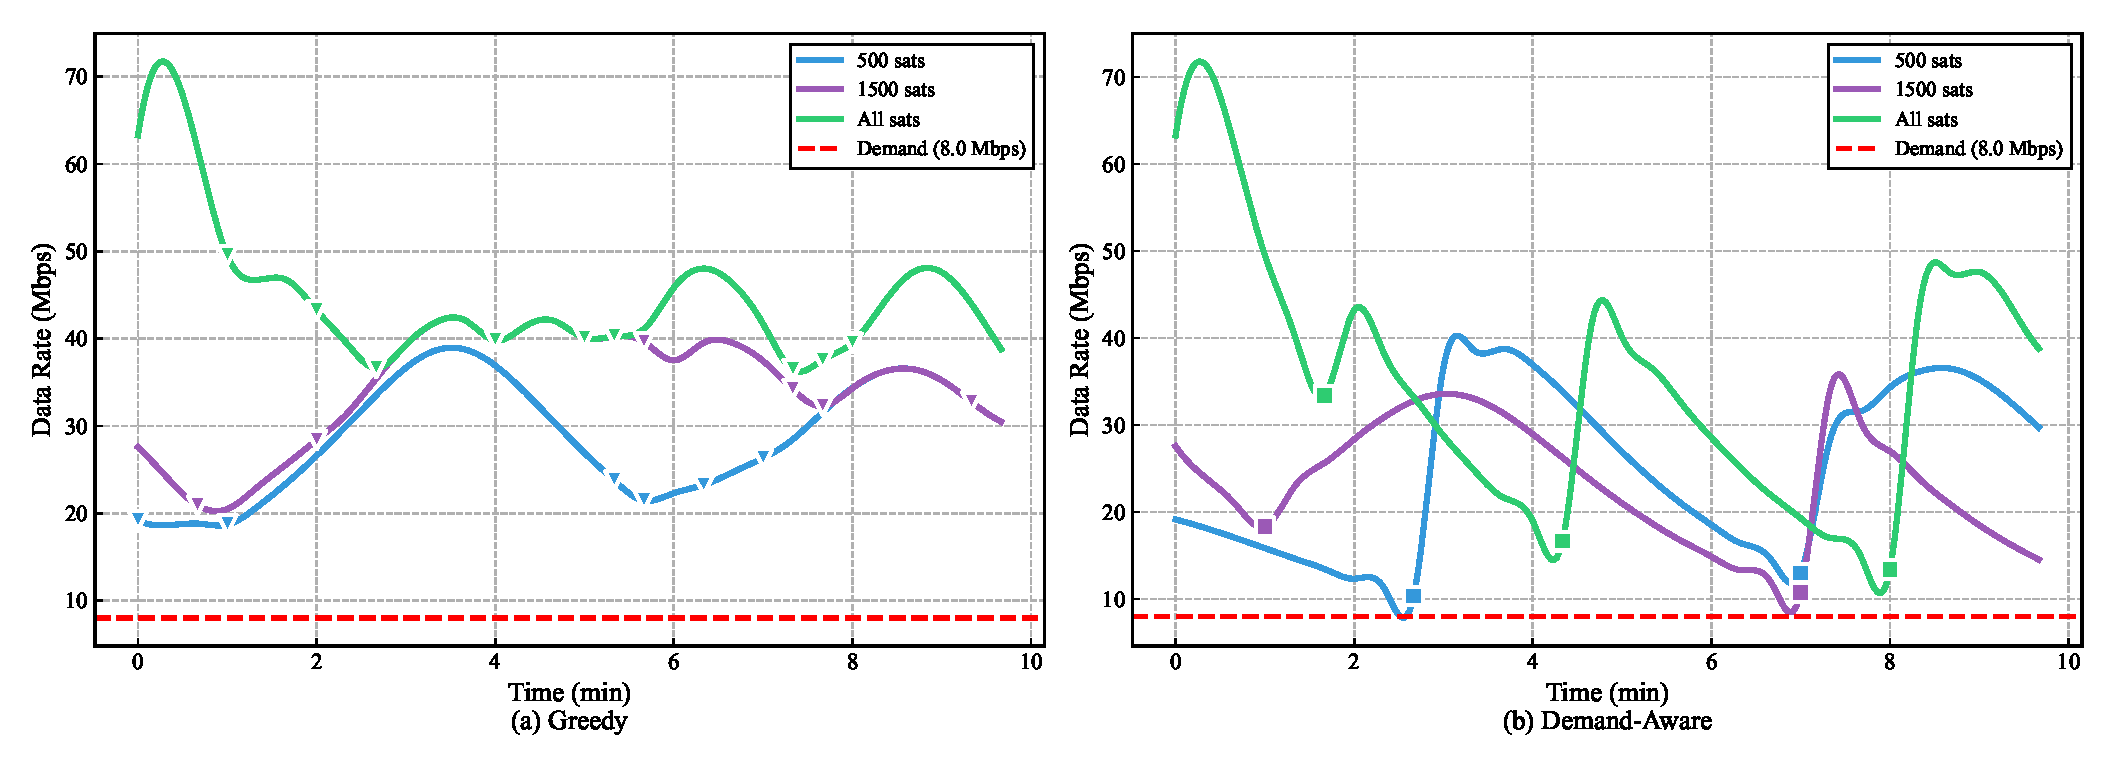
\includegraphics[width=0.95\textwidth]{Definitions/demand_aware_number_of_satellites}
\caption{Data rate comparison between Greedy and Demand-Aware strategies across different satellite densities: (a) Greedy strategy exhibits frequent rate fluctuations and numerous handovers (marked with triangles), pursuing maximum instantaneous throughput, while (b) Demand-Aware strategy maintains stable rates above the 8~Mbps demand threshold (red dashed line) with significantly fewer handovers (marked with squares), switching only when necessary to meet transmission requirements.}
\label{fig:demand_aware_satellites}
\end{figure*}

In contrast, the Demand-Aware strategy in Fig.~\ref{fig:demand_aware_satellites}(b) demonstrates remarkably stable behavior. The data rates remain consistently above the 8~Mbps demand threshold (indicated by the red dashed line) throughout the entire mission, with only 2-3 handovers across all scenarios. The rate stability is particularly evident in the 500-satellite case, where Demand-Aware maintains smooth rate curves with minimal fluctuations despite having fewer satellites available. This stability arises from the algorithm's conservative switching policy: as long as the current satellite can deliver sufficient throughput to complete the remaining data transmission within the available time window, no handover is triggered. Only when the predicted future capacity becomes inadequate does the algorithm proactively switch to a better candidate.

The quantitative handover analysis in Fig.~\ref{fig:packet_loss}(a) reveals the dramatic difference in switching behavior. For the 500-satellite scenario, Demand-Aware reduces handovers from 7 (Greedy) to just 2, representing a 71.4\% reduction. This improvement persists across all constellation densities: 75.0\% reduction for 1500 satellites (from 8 to 2) and 66.7\% reduction for the full constellation (from 9 to 3). Notably, the Demand-Aware handover count remains remarkably stable regardless of satellite density---consistently between 2 and 3---while the Greedy count increases with constellation size as more switching opportunities become available. This stability demonstrates that Demand-Aware bases decisions on transmission requirements rather than merely responding to instantaneous channel conditions.

% Figure 4: Handover and packet loss analysis
\begin{figure}[!t]
\centering
\includegraphics[width=0.95\columnwidth]{Definitions/packet_loss_analysis}
\caption{Handover frequency and packet loss comparison: (a) Demand-Aware achieves 66.7--75.0\% handover reduction across all satellite densities, with the most significant improvement (75.0\%) in the 1500-satellite scenario, (b) Corresponding packet loss rates show proportional reduction, with Demand-Aware maintaining remarkably low loss rates of 0.133--0.200\% compared to 0.467--0.600\% for Greedy.}
\label{fig:packet_loss}
\end{figure}

The reduction in handover frequency directly translates to improved packet delivery performance, as shown in Fig.~\ref{fig:packet_loss}(b). The packet loss rate is calculated based on the 400~ms handover delay: each handover causes a 400~ms service interruption during which transmitted packets are lost. For a 10-minute mission, the packet loss rate is computed as (Number of Handovers $\times$ 400~ms) / (600~s $\times$ 1000~ms) $\times$ 100\%. In the 500-satellite scenario, Demand-Aware achieves a packet loss rate of only 0.133\%, compared to 0.467\% for Greedy---a 71.4\% reduction. The most dramatic improvement occurs in the 1500-satellite case, where packet loss drops from 0.533\% to 0.133\%, representing a 75.0\% reduction. These seemingly small percentages translate to significant practical impact: at an 8~Mbps data rate, a 0.533\% loss rate means approximately 42.6~kbit of lost data over 10 minutes, compared to just 10.6~kbit for Demand-Aware. For latency-sensitive applications such as real-time video streaming or industrial control, this reliability improvement is crucial.

An important trade-off emerges when comparing average data rates. The Greedy strategy achieves higher average throughput: 28.62~Mbps for 500 satellites, 34.29~Mbps for 1500 satellites, and 44.78~Mbps for the full constellation. In comparison, Demand-Aware obtains 24.87~Mbps, 23.37~Mbps, and 35.27~Mbps, respectively---representing 13.1\% to 31.8\% lower average rates. However, this throughput sacrifice must be evaluated in context. The demand rate is set to 8~Mbps, and Demand-Aware consistently delivers 3$\times$ to 4$\times$ this requirement. The excess capacity provides a comfortable margin for handling temporary channel degradation without triggering handovers. Meanwhile, Greedy's pursuit of maximum throughput comes at the cost of 200--300\% higher packet loss and more frequent service interruptions. For most applications, meeting the demand threshold reliably is more valuable than maximizing peak throughput at the expense of stability.

The scalability characteristics across constellation densities reveal contrasting behaviors. Greedy's handover count increases moderately with satellite density (+28.6\% from 500 to full constellation), as more satellites create more switching opportunities. This trend is problematic because future LEO deployments will feature increasingly dense constellations, potentially exacerbating the handover problem. Conversely, Demand-Aware maintains consistently low handover counts (2--3) regardless of density, demonstrating excellent scalability. The algorithm's switching decisions depend on whether current capacity can meet remaining demand, not on how many alternative satellites are visible. This fundamental design difference makes Demand-Aware naturally robust to constellation density variations.

The performance in the 500-satellite scenario deserves particular attention as it represents the optimal operating point for Demand-Aware. With only 2 handovers and a packet loss rate of just 0.133\%, the system achieves exceptional stability while maintaining an average rate of 24.87~Mbps---more than sufficient for the 8~Mbps demand. This suggests that moderate satellite density may be preferable to maximum density for stability-critical applications. The 1500-satellite scenario also performs excellently with identical handover count (2) and packet loss (0.133\%), indicating that Demand-Aware can leverage increased satellite availability to maintain quality without triggering excessive switching.

% ==============================================================================
% 4.4 End-to-End System Analysis
% ==============================================================================

\subsection{End-to-End System Analysis}

The preceding subsections have demonstrated the effectiveness of Algorithm 1 in minimizing UAV energy consumption during IoT data collection and Algorithm 2 in reducing handover frequency during satellite offloading. However, the true value of our framework lies in the synergistic integration of these two stages into a cohesive end-to-end system. To fully appreciate this synergy, we now examine how the algorithms work together to optimize overall mission performance from ground-based IoT devices to cloud-based processing infrastructure.

Consider a representative mission scenario with $K=50$ IoT devices and 500 visible LEO satellites. In the first stage, the proposed Adam-2opt algorithm collects data from all IoT devices using optimized trajectories, consuming 38,789.84~J of UAV energy over a flight distance of 2,854.92~m. The data collection completes with 25 hovering points serving 22 paired devices, taking approximately $T_{\text{collect}} = T_{\text{hover}} + T_{\text{flight}} = 56.64 + (2854.92/10) = 342.13$~s, assuming a typical UAV flight speed of 10~m/s. At this point, the UAVs have aggregated the IoT data and are ready to begin the second stage.

In the second stage, the UAVs offload their aggregated data to LEO satellites using the Demand-Aware handover strategy. With an average data rate of 24.87~Mbps and only 2 handovers occurring over the 10-minute observation window, the system achieves stable connectivity with minimal service interruptions. The packet loss rate of 0.133\% ensures that virtually all collected data successfully reaches the cloud. Comparing this integrated performance against a baseline system using Random Pairing for Stage 1 and Greedy for Stage 2 reveals the comprehensive advantages of our approach: 16.6\% reduction in UAV energy consumption, 71.4\% reduction in satellite handovers, and 71.4\% reduction in packet loss---all achieved simultaneously.

The key insight is that optimizing each stage independently is insufficient; the stages must be designed with complementary objectives. Algorithm 1 focuses on spatial efficiency (minimizing flight distance and hovering time) while Algorithm 2 emphasizes temporal stability (minimizing switching frequency). These objectives are naturally compatible: efficient data collection reduces the total data volume that must be offloaded, which in turn reduces the transmission time required and allows the Demand-Aware strategy to maintain stable connections with fewer handovers. Conversely, stable satellite connectivity reduces the risk of transmission failures that would otherwise require retransmission and additional UAV energy expenditure.

Table~\ref{tab:end_to_end_comparison} summarizes the end-to-end performance metrics for the complete system. The proposed two-stage framework achieves substantial improvements across all dimensions compared to baseline combinations. The 16.6\% UAV energy reduction directly extends mission duration and operational range, critical factors for battery-constrained UAVs. The 71.4\% handover reduction minimizes service interruptions and signaling overhead, which is particularly valuable for latency-sensitive applications. The 71.4\% packet loss reduction ensures reliable data delivery even under dynamic channel conditions. While the average data rate is 13.1\% lower than the Greedy approach, this trade-off is well-justified given that the achieved rate (24.87~Mbps) exceeds the demand requirement (8~Mbps) by a factor of 3$\times$, providing ample margin for handling temporary channel degradation.

\begin{table}[!t]
\centering
\caption{End-to-End System Performance Comparison ($K=50$, 500 Satellites)}
\label{tab:end_to_end_comparison}
\begin{tabular}{lccc}
\toprule
\textbf{Metric} & \textbf{Baseline} & \textbf{Proposed} & \textbf{Improvement} \\
\midrule
UAV Energy (J) & 46,490.88 & 38,789.84 & $-16.6\%$ \\
Flight Distance (m) & 3,088.77 & 2,854.92 & $-7.6\%$ \\
Collection Time (s) & 426.70 & 342.13 & $-19.8\%$ \\
\midrule
Handover Count & 7 & 2 & $-71.4\%$ \\
Packet Loss (\%) & 0.467 & 0.133 & $-71.4\%$ \\
Avg. Data Rate (Mbps) & 28.62 & 24.87 & $-13.1\%$ \\
\bottomrule
\multicolumn{4}{l}{\footnotesize Baseline: Random Pairing + Greedy; Proposed: Adam-2opt + Demand-Aware}
\end{tabular}
\end{table}

The scalability analysis across varying IoT device densities reveals interesting trends in end-to-end performance. At small network sizes ($K=20$), the energy advantage of Algorithm 1 is modest (1.3\% improvement), as baseline methods already perform reasonably well when the problem complexity is limited. However, the handover reduction from Algorithm 2 remains substantial (71.4\%) even at this scale, indicating that the satellite selection problem is inherently challenging regardless of ground network size. As the network scales to $K=50$, the energy savings increase dramatically to 16.6\%, demonstrating that sophisticated trajectory optimization becomes increasingly valuable in dense deployments. Importantly, the handover reduction remains stable across all device densities, confirming that Algorithm 2's performance is robust to variations in the ground segment workload. This independent scalability of the two stages is a desirable property: Algorithm 1 adapts to ground network complexity while Algorithm 2 maintains consistent performance in the space segment.

The robustness of the system to satellite density variations further validates our design approach. While Greedy's handover count increases with constellation size (from 7 to 9 as satellites increase), Demand-Aware maintains consistently low handover counts (2--3) across all densities. This behavior ensures that the system will perform well even as LEO constellations continue to expand in future deployments. The proposed framework demonstrates a fundamental principle: satisfying operational requirements with minimal resource consumption is often superior to maximizing instantaneous performance metrics at the cost of stability and efficiency.

%%%%%%%%%%%%%%%%%%%%%%%%%%%%%%%%%%%%%%%%%%
\section{Discussion}

The simulation results presented in this section reveal several important insights into the design of efficient UAV-assisted IoT data collection and LEO satellite offloading systems. Beyond the quantitative performance improvements, the experiments illuminate fundamental principles that should guide future system designs in SAGIN environments.

The success of Algorithm 1 demonstrates that effective UAV trajectory optimization requires simultaneous consideration of multiple coupled objectives. Optimizing only hovering positions, as in Basic Optimization, yields suboptimal results because it ignores the flight path structure. Similarly, minimizing hovering time alone, as in Fixed Hovering, leads to excessive flight distance. Our Adam-2opt approach achieves superior performance by recognizing that these objectives are fundamentally interrelated: the optimal hovering positions depend on the trajectory that connects them, and the optimal trajectory depends on where the hovering points are located. The Adam optimizer provides fine-grained position adjustments through gradient-based updates, while 2-opt refines the trajectory structure through combinatorial search. This hybrid approach combines the strengths of continuous optimization and discrete search, yielding better solutions than either technique alone.

The Demand-Aware handover strategy embodies a paradigm shift in satellite network optimization. Traditional approaches, exemplified by the Greedy baseline, focus on maximizing instantaneous performance metrics such as data rate or signal strength. This myopic perspective fails to account for the long-term consequences of frequent switching: handover delays, packet loss, signaling overhead, and degraded user experience. Our Demand-Aware strategy adopts a fundamentally different philosophy: determine the minimum requirements to complete the mission successfully, and avoid unnecessary actions that would jeopardize stability. This principle of \textit{sufficiency-based optimization}---doing just enough to meet the objective without over-optimizing secondary metrics---proves remarkably effective. By maintaining connections that satisfy demand requirements rather than chasing peak throughput, the algorithm achieves 66.7--75.0\% handover reduction while still delivering 3$\times$ the required data rate.

The synergy between the two algorithms highlights a critical insight for multi-stage system design: the objectives optimized in different stages should be complementary rather than competing. Algorithm 1 minimizes UAV energy by reducing spatial inefficiencies (flight distance, hovering time), while Algorithm 2 minimizes handover overhead by reducing temporal instability (switching frequency, service interruptions). These objectives align naturally: energy-efficient data collection reduces the transmission burden in the offloading stage, and stable satellite connectivity reduces the risk of retransmission that would otherwise waste UAV energy. This complementary design ensures that optimizing one stage does not inadvertently degrade the other.

Comparing our approach to potential alternatives reveals important trade-offs. One might ask: why not use a single integrated optimization that jointly optimizes UAV trajectories and satellite handovers? While theoretically appealing, such an approach would face severe computational challenges due to the vastly different timescales and dynamics of the two stages. UAV trajectory planning operates on minutes-to-hours timescales with relatively static device positions, allowing for offline pre-computation. Satellite handover decisions must be made in real-time (seconds) based on rapidly changing orbital dynamics. Combining these problems would either force the trajectory optimizer to account for unpredictable future satellite positions (intractable) or require the handover algorithm to wait for trajectory recomputation (impractical). Our two-stage approach respects these temporal separations while still achieving strong overall performance.

The trade-off between energy efficiency and computational complexity also merits discussion. The proposed Adam-2opt algorithm requires 1.2024 seconds of computation time for $K=50$ devices, significantly longer than the 0.0613 seconds needed by Basic Optimization. However, this overhead is well-justified in the context of offline mission planning. UAV missions are typically planned hours or days in advance, and a few additional seconds of planning time is negligible compared to the mission duration (typically 30--60 minutes). The 16.6\% energy savings translate directly to extended mission range or longer operational time, both of which are far more valuable than saving one second of pre-flight computation. For applications requiring real-time replanning due to dynamic events (sudden device failures, obstacle avoidance), faster approximation algorithms could be substituted, though at some cost to solution quality.

The observed scalability trends suggest that our approach becomes increasingly valuable as SAGIN systems expand. The 16.6\% energy improvement at $K=50$ devices, compared to just 1.3\% at $K=20$, indicates that sophisticated optimization techniques are most beneficial precisely when they are most needed---in large-scale deployments where naive approaches break down. Similarly, the consistent handover reduction (66.7--75.0\%) across all satellite densities confirms that Demand-Aware will continue to perform well as LEO constellations grow denser. This combination of strong baseline performance and excellent scaling behavior positions our framework as a robust solution for both current and future SAGIN deployments.

Several practical considerations arise when contemplating real-world deployment. For Algorithm 1, the assumption of perfect channel state information should be relaxed in practice. Actual implementations would need to estimate channel gains from pilot signals and incorporate prediction errors into the optimization. The single-visit constraint could also be relaxed to allow multiple UAV passes over the coverage area, trading increased mission time for better energy efficiency. For Algorithm 2, the fixed demand threshold could be replaced with an adaptive mechanism that adjusts based on observed channel conditions and remaining mission time. The algorithm could also be extended to coordinate handovers across multiple UAVs to avoid simultaneous switching events that might overwhelm satellite resources.

Despite these potential enhancements, the current framework already demonstrates strong practical viability. The algorithms require no specialized hardware beyond standard UAV platforms and commodity satellite transceivers. The computational requirements are modest enough for embedded flight computers. The performance improvements are substantial enough to justify implementation effort. Most importantly, the framework is modular: the two stages can be deployed independently, allowing operators to adopt whichever component best addresses their primary bottleneck.

%%%%%%%%%%%%%%%%%%%%%%%%%%%%%%%%%%%%%%%%%%
\section{Conclusions}

In this paper, we address the data collection and offloading problem by integrating UAVs trajectories planning and LEO satellite selection in SAGIN. The problem is formulated to minimize the energy consumption with the constraints on multi-dimension variables. Specifically, in the data collection  phase from IoT to UAV, the algorithm is designed to optimize the IoT pairing, power optimization, UAV trajectory planning. In the data offloading phase from UAV to LEO, a real-time LEO satellite selection mechanism joint with STK is proposed. Finally, simulation results verified the effectiveness of the proposed approach, with about 10\% less energy consumption compared with the benchmark algorithm.
oilk,
%%%%%%%%%%%%%%%%%%%%%%%%%%%%%%%%%%%%%%%%%%
%\isPreprints{} % If the paper is ``preprints'', please uncomment this parenthesis.
%\printendnotes[custom] % Un-comment to print a list of endnotes

\reftitle{References}

% Please provide the correct journal abbreviation (e.g. according to the “List of Title Word Abbreviations” http://www.issn.org/services/online-services/access-to-the-ltwa/).
% Citations and References in Supplementary files are permitted provided that they also appear in the reference list here. 

%=====================================
% References, variant A: external bibliography
%=====================================
% \bibliography{your_external_BibTeX_file}

%=====================================
% References, variant B: internal bibliography
%=====================================

% ACS format
\begin{thebibliography}{999}
% Reference 1
\bibitem{jia2020leo}
Jia, Z.; Sheng, M.; Li, J.; Niyato, D.; Han, Z.
LEO-satellite-assisted UAV: Joint trajectory and data collection for Internet of Remote Things in 6G aerial access networks.
{\em IEEE Internet Things J.} {\bf 2020}, {\em 8}, 9814--9826.

% Reference 2
\bibitem{xiao2024space}
Xiao, Y.; Ye, Z.; Wu, M.; Li, H.; Xiao, M.; Alouini, M.-S.; Al-Hourani, A.; Cioni, S.
Space-air-ground integrated wireless networks for 6G: Basics, key technologies and future trends.
{\em IEEE J. Sel. Areas Commun.} {\bf 2024}.

% Reference 3
\bibitem{duan2022distributed}
Duan, S.; Wang, D.; Ren, J.; Lyu, F.; Zhang, Y.; Wu, H.; Shen, X.
Distributed artificial intelligence empowered by end-edge-cloud computing: A survey.
{\em IEEE Commun. Surv. Tutor.} {\bf 2022}, {\em 25}, 591--624.

% Reference 4
\bibitem{wei2024energy}
Wei, Q.; Chen, Y.; Jia, Z.; Bai, W.; Pei, T.; Wu, Q.
Energy-efficient caching and user selection for resource-limited SAGINs in emergency communications.
{\em IEEE Trans. Commun.} {\bf 2024}.

% Reference 5
\bibitem{pan2022latency}
Pan, G.; Ye, J.; An, J.; Alouini, M.-S.
Latency versus reliability in LEO mega-constellations: Terrestrial, aerial, or space relay?
{\em IEEE Trans. Mob. Comput.} {\bf 2022}, {\em 22}, 5330--5345.

% Reference 6
\bibitem{jia2025distributionally}
Jia, Z.; Cui, C.; Dong, C.; Wu, Q.; Ling, Z.; Niyato, D.; Han, Z.
Distributionally robust optimization for aerial multi-access edge computing via cooperation of UAVs and HAPs.
{\em IEEE Trans. Mob. Comput.} {\bf 2025}.

% Reference 7
\bibitem{mao2020joint}
Mao, S.; He, S.; Wu, J.
Joint UAV position optimization and resource scheduling in space-air-ground integrated networks with mixed cloud-edge computing.
{\em IEEE Syst. J.} {\bf 2020}, {\em 15}, 3992--4002.

% Reference 8
\bibitem{zhao2021multi}
Zhao, C.; Liu, J.; Sheng, M.; Teng, W.; Zheng, Y.; Li, J.
Multi-UAV trajectory planning for energy-efficient content coverage: A decentralized learning-based approach.
{\em IEEE J. Sel. Areas Commun.} {\bf 2021}, {\em 39}, 3193--3207.
% Reference 9
\bibitem{mozaffari2019tutorial}
Mozaffari, M.; Saad, W.; Bennis, M.; Nam, Y.-H.; Debbah, M.
A tutorial on UAVs for wireless networks: Applications, challenges, and open problems.
{\em IEEE Commun. Surv. Tutor.} {\bf 2019}, {\em 21}, 2334--2360.
% Reference 10
\bibitem{tao2015survey}
Tao, Y.; Liu, L.; Liu, S.; Zhang, Z.
A survey: Several technologies of non-orthogonal transmission for 5G.
{\em China Commun.} {\bf 2015}, {\em 12}, 1--15.
% Reference 11
\bibitem{fang2022noma}
Fang, X.; Feng, W.; Wang, Y.; Chen, Y.; Ge, N.; Ding, Z.; Zhu, H.
NOMA-based hybrid satellite-UAV-terrestrial networks for 6G maritime coverage.
{\em IEEE Trans. Wireless Commun.} {\bf 2022}, {\em 22}, 138--152.
% Reference 12
\bibitem{jia2025service}
Jia, Z.; Cao, Y.; He, L.; Wu, Q.; Zhu, Q.; Niyato, D.; Han, Z.
Service function chain dynamic scheduling in space-air-ground integrated networks.
{\em IEEE Trans. Veh. Technol.} {\bf 2025}.
% Reference 13
\bibitem{huang2024joint}
Huang, C.; Chen, G.; Xiao, P.; Xiao, Y.; Han, Z.; Chambers, J. A.
Joint offloading and resource allocation for hybrid cloud and edge computing in SAGINs: A decision assisted hybrid action space deep reinforcement learning approach.
{\em IEEE J. Sel. Areas Commun.} {\bf 2024}, {\em 42}, 1029--1043.
% Reference 14
\bibitem{jia2024dynamic}
Jia, H.; Wang, Y.; Wu, W.
Dynamic resource allocation for remote IoT data collection in SAGIN.
{\em IEEE Internet Things J.} {\bf 2024}, {\em 11}, 20575--20589.
% Reference 15
\bibitem{seyedi2012trace}
Seyedi, Y.; Rahimi, F.
A trace-time framework for prediction of elevation angle over land mobile LEO satellites networks.
{\em Wirel. Pers. Commun.} {\bf 2012}, {\em 62}, 793--804.
% Reference 16
\bibitem{d2020learning}
d O Costa, P. R.; Rhuggenaath, J.; Zhang, Y.; Akcay, A.
Learning 2-opt heuristics for the traveling salesman problem via deep reinforcement learning.
{\em Asian Conf. Mach. Learn.} {\bf 2020}, 465--480.

\end{thebibliography}

% If authors have biography, please use the format below
%\section*{Short Biography of Authors}
%\bio
%{\raisebox{-0.35cm}{\includegraphics[width=3.5cm,height=5.3cm,clip,keepaspectratio]{Definitions/author1.pdf}}}
%{\textbf{Firstname Lastname} Biography of first author}
%
%\bio
%{\raisebox{-0.35cm}{\includegraphics[width=3.5cm,height=5.3cm,clip,keepaspectratio]{Definitions/author2.jpg}}}
%{\textbf{Firstname Lastname} Biography of second author}

% For the MDPI journals use author-date citation, please follow the formatting guidelines on http://www.mdpi.com/authors/references
% To cite two works by the same author: \citeauthor{ref-journal-1a} (\citeyear{ref-journal-1a}, \citeyear{ref-journal-1b}). This produces: Whittaker (1967, 1975)
% To cite two works by the same author with specific pages: \citeauthor{ref-journal-3a} (\citeyear{ref-journal-3a}, p. 328; \citeyear{ref-journal-3b}, p.475). This produces: Wong (1999, p. 328; 2000, p. 475)

%%%%%%%%%%%%%%%%%%%%%%%%%%%%%%%%%%%%%%%%%%
%% for journal Sci
%\reviewreports{\\
%Reviewer 1 comments and authors’ response\\
%Reviewer 2 comments and authors’ response\\
%Reviewer 3 comments and authors’ response
%}
%%%%%%%%%%%%%%%%%%%%%%%%%%%%%%%%%%%%%%%%%%
\begin{comment}
\PublishersNote{}
\end{comment}
%\isPreprints{} % If the paper is ``preprints'', please uncomment this parenthesis.

\end{document}


